\documentclass[letterpaper]{report}
\usepackage[utf8]{inputenc}
\usepackage{setspace}
\usepackage{geometry}
\usepackage{graphicx}
\usepackage{svg}
\usepackage{amsmath}
\usepackage{wrapfig}

%for fancy quotes
\usepackage{epigraph}

% allow hyperlinks
\usepackage{hyperref}
\usepackage{caption}
\hypersetup{
    colorlinks=true,
    linkcolor=blue,
    filecolor=magenta,      
    urlcolor=cyan,
    pdftitle={SOEN 6461 Winter 2023 D1 Team N},
    pdfpagemode=FullScreen,
    }
\urlstyle{same}
\usepackage[inline]{enumitem}

\usepackage{authblk}

\begin{document}

\begin{titlepage}
\newcommand{\HRule}{\rule{\linewidth}{0.5mm}} % Defines a new command for the horizontal lines, change thickness here

%	LOGO SECTION
\center % Center everything on the page

\includegraphics[width=14cm]{concordia-logo.jpg} % Include a department/university logo - this will require the graphicx package
\vspace{\baselineskip}
\vspace{0.8cm}


%	HEADING SECTIONS

\oddsidemargin=20pt
\setstretch{1.30} \textsc{\LARGE SOEN 6461 
\\ SOFTWARE DESIGN METHODOLOGIES} \\[1.4cm]
\textsc{\Large Concordia University}\\[0.5cm]
\textsc{\large Department of Computer Science and Software Engineering}\\[0.5cm]


%	TITLE SECTION

\title{\Large iGo Ticket Vending Machine - Deliverable 1}
\makeatletter
\HRule \vspace{0.4cm}
{ \huge \bfseries \@title} \\ % Title of your document
\vspace{0.2cm} 
\HRule \vspace{1.1cm}
\makeatother

%	AUTHOR SECTION
\Large \emph{Authors (Team N):}\\
\item Swapnil Kamleshkumar Rana \hspace{0.8cm} Kevin Rao \hspace{0.8cm} Himanshu Rathod \item Elvin Rejimone \hspace{0.8cm} Sadath Roshan

\vspace {1.8cm}
%	DATE SECTION
 {\large March 6, 2023}

\end{titlepage}
\tableofcontents
\listoffigures
\listoftables

\chapter{Problem 1 : Project Description}
\epigraph{Land was created to provide a place for boats to visit. }{\textit{Brooks Atkinson}}
\vspace{\baselineskip}
View the source code of the report \href{https://www.overleaf.com/read/jdwsnqmxksty}{here [read-only]}.\\
Roles and responsibilities were distributed amongst the team members, they are viewable \href{https://docs.google.com/document/d/1j38J-lBybRq45DPbRcwjgABt5lwJG8n9n4gw6vJoOlY/}{here}.
\section{Ticket Vending Machine}

A Ticket Vending Machine (TVM), also known as a ticket machine or a ticketing kiosk, 
is an automated, self-service, vending machine that produces paper or electronic tickets, or recharges a stored-value card or online wallet for a multitude of purposes like Transportation, Mobile recharge or theme park entrances. 

\section{iGo : Project Description}
The purpose of the project is to create a Ticket Vending Machine we refer to as iGo for a public transport service legally permitted in Canada. The transportation service selected for iGo is the Montréal Ferry System(Navette Maritimes) that operates in ports along the Saint Lawrence River and along the river to ports in a few nearby cities mentioned later in the document. The Ticket Vending Machines (iGo) localted in all ports of service is intended to be the only ticketing system to provide commuters with the tickets to use the Ferry Services.

\subsection{Details of the Transportation Service Considered : Montréal Ferry System}
The Montréal Ferry System(Navette Maritimes) is a public Ferry service that services multiple locations, including Montréal's Old Port, Parc-Jean Dreupue, and Longueuil. The Service also provides intercity ferry-travel to Ottawa, Quebec City, Toronto, and Kingston. The iGo software will be designed to be maintainable, secure, environmentally sustainable, and usable. It will be built using a combination of agile and rigid methodologies and will involve both individual and communal work. The iGo ticket vending machine will provide a convenient and efficient way for passengers to purchase their travel ticket.

\subsubsection{Port Stations}
\begin{itemize}
    \item \textbf{Montréal Stations }
    \begin{itemize}
        \item Montréal Old Port 
        \item Longueuil - Departure from Longueuil Marina
        \item Parc Jean-Drepeau - Stewart Museum
    \end{itemize}
    \item \textbf{Inter-city Stations}
    \begin{itemize}
        \item Montréal Old port
        \item Toronto
        \item Ottawa
        \item Quebec City
        \item Kingston
    \end{itemize}
\end{itemize}

\subsubsection{Service Details}  
There will be multiple Ticket Vending Machines at the every port given in the above list. 
There are two types of ferry services: -
\begin{itemize}
    \item Short-distance Ferry (Longueuil, Parc Jean Drapeau, Old Port) (Within Montréal)
    \item Long-distance Ferry (Toronto, Ottawa, Quebec City, Kingston,  (Outside Montréal)
\end{itemize}
\subsubsection{Types of Tickets}
\begin{itemize}
    \item Single-use tickets - \$5.50 (consume one per direction)
    \item Return trip tickets - \$7 (consume one for two directions)
    \item Day pass tickets - \$10 (consume one per day)
    \item Recreational ticket - \$20 (ferry makes a circle, starts and end at same station)
    \item Ticket option for car.( People sitting in the car do not need a personal ticket). 
\begin{itemize}
    \item Cars with up to 5 seats - \$15
    \item Cars with 7/8  seats -  \$20
\end{itemize}
    \item Long-Distance Ticket (Price depends on the destination) 
\end{itemize}

\subsection{Scope of the Project: iGo Ticket Vending Machine}
The scope of this project is to design and develop the iGo Ticket Vending Machine for the above mentioned Montréal Ferry Service. The scope includes full ticket booking(for Montréal Ferry and Inter-city ferry) operation in the TVM , Payment initiation, payment confirmation and the physical ticket printing. It does not cover the operations performed by the Server, Bank or any other system not physically in the Vending Machine. 
\subsubsection{Operations required to be performed by iGo TVM}
\begin{itemize}
    \item Ferry Ticketing
     \begin{itemize}
        \item Montréal Ferry ticket
        \item Inter-city Ferry ticket
    \end{itemize}
    \item Ticket Confirmation
    \item Payment 
    \begin{itemize}
        \item Payment by Cash
        \item Payment by Card (Debit/Credit/Bank Cards)
    \end{itemize}
    \item Print Ticket
    \item On-site Booking Assistance for Commuters 
\end{itemize}
\vspace{\baselineskip}

In the following sections we will be discussing the problem domain with package diagrams, mind-mapping for the project, several interviews with potential users to obtain valuable insights and conclusions, create a use-case model and several activity diagrams to aid in the development of the iGo Ticket Vending Machine,

\chapter{Problem 2}
Refer to figure \ref{fig:problemDomain} and figure \ref{fig:problemPackage} for the problem domain model diagram and its package diagram. The figures were created using lecture slides by Pankaj Kamthan\cite{DomainModelDiagramming} as a guide. The classes, their attributes, and the relationship between these will be defined subsequently. Their definitions will be organized by the package the class is categorized in. View the figures \href{https://drive.google.com/file/d/1l209HYuvMnJnniDuLFu2vUxGI3H7XldU/view?usp=sharing}{here}.

\begin{figure}[ht] %h means try putting the figure here and t means try putting it at the top of a subsequent page. ht mean try h first, then t.
    \centering
    % \includesvg{ProblemDomainDiagram/Problem Domain Model-Package Diagram of Problem Domain Model.svg} %svg has problems rendering, for whatever reason.
    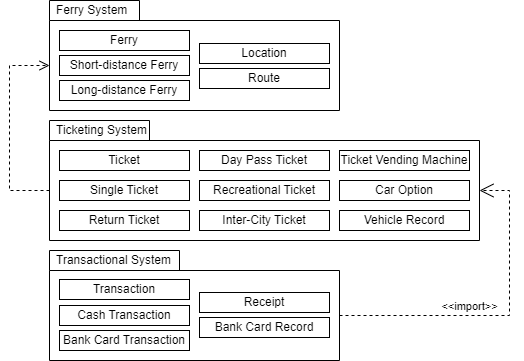
\includegraphics[width=\textwidth]{ProblemDomainDiagram/Problem Domain Model-Package Diagram of Problem Domain Model.png}
    \caption{Package Diagram of Problem Domain Model}
    \label{fig:problemPackage}
\end{figure}
\begin{figure}[ht]
    \centering
    % \includesvg[width=\textwidth]{ProblemDomainDiagram/Problem Domain Model-Problemin Model.svg} %svg has problems rendering, for whatever reason.
    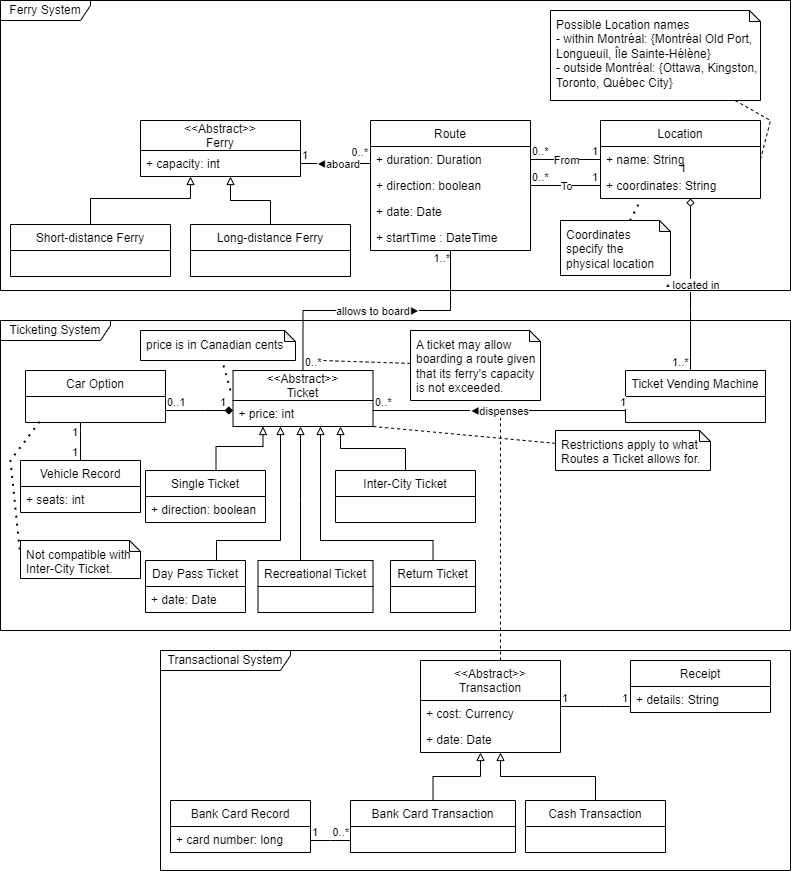
\includegraphics[width=\textwidth]{ProblemDomainDiagram/Problem Domain Model-Problem Domain Model.png}
    \caption{Diagram of Problem Domain Model}
    \label{fig:problemDomain}
\end{figure}
\clearpage  %print all figures.
\section{Ferry System package}
\subsection{Class Descriptions}
\begin{itemize}
    \item Location class represents physical locations for which a ferry will travel between. Its attributes are the common name of the physical location and its longitude and latitude coordinates to uniquely identify the space where it can be found. Locations are either within or outside Montréal.
    \item Route class is the ternary relationship between a from-Location, a to-Location and a Ferry. The Route starts from the from-Location, and ends at the to-Location. The Route will be aboard the Ferry from one Location to another (or the same) Location. About its attributes, a route travels in a direction (West or East), with a planned startTime for a planned duration on a particular date. At least one of the Locations must be within Montréal.
    \item Ferry class represents the physical ferry that will be travelled on. About its attributes, it has a maximum capacity of passengers. 
    \item Short-distance Ferry is a concrete Ferry that can only travel for Routes that are between Locations within Montréal.
    \item Long-distance Ferry is a concrete Ferry that can only travel for Routes that are between one Location within Montréal and one Location outside Montréal.
\end{itemize}

\subsection{Relationship Multiplicity Justifications}
\begin{itemize}
    \item {[Between Location and Route]} A Location may serve as a from-/to-Location to multiple Routes or to no Routes, but a Route must only have one from-Location and one to-Location.
    \item {[Between Ferry and Route]} A Route must be conducted aboard one Ferry. A Ferry may be used for multiple or no Routes.
\end{itemize}

\section{Ticketing System package}
\subsection{Class Descriptions}
The classes will be further partitioned by the roles they occupy.
\subsubsection{Ticket Kinds}
\begin{itemize}
    \item Ticket class allows permission to board a Route’s Ferry. Its attribute is the price in Canadian cents (ints are more precise in handling currencies with decimals than floats) associated with purchasing the Ticket. There is the option to board a Ferry with a vehicle.
    \item Single Ticket is a concrete Ticket that allows passage along a set of Routes in the same direction starting from the Location it has been dispensed from. Its attribute is the direction of Routes this Ticket allows to board. It only allows to board Routes aboard a Short-distance Ferry, and does not allow boarding Routes whose to-/from-Locations are the same..
    \item Return Ticket is a concrete Ticket that allows passage along a set of Routes in the same direction, followed by another set of Routes in the opposite direction. In practice, this should allow a commuter to travel in one direction, then later come back to his initial location with only this Ticket. It only allows to board Routes aboard a Short-distance Ferry, and does not allow boarding Routes whose to-/from-Locations are the same.
    \item Day Pass Ticket is a concrete Ticket that allows passage along a set of Routes on one day. Its attribute is the day all Routes can be boarded with this Ticket. It only allows to board Routes aboard a Short-distance Ferry, and does not allow boarding Routes whose to-/from-Locations are the same.
    \item Recreational Ticket is a concrete Ticket that allows passage on a single Route whose to-/from-Locations are the same. It only allows to board Routes aboard a Short-distance Ferry.
    \item InterCity Ticket is a concrete Ticket that allows passages on a single Route aboard a Long-distance Ferry.
\end{itemize}

\subsubsection{Ticket Decorator}
\begin{itemize}
    \item Car Option class lets a Ticket allow the transport of a Vehicle along its Route, except for Inter-City Tickets. This option also allows passage for as many commuters as there are seats to the vehicle. A Car Option must have an associated Vehicle Record to be valid. Having a Car Option modifies the price of the Ticket.
    \item Vehicle Record class represents the bureaucratic paperwork as proof for a vehicle to be assigned to a particular Car Option. Its attribute is the number of seats the vehicle is documented to support.
\end{itemize}

\subsubsection{Ticket Dispenser}
\begin{itemize}
    \item Ticket Vending Machine class represents the iGo TVM to be installed at a Location to dispense Tickets.
\end{itemize}

\subsection{Relationship Multiplicity Justifications}
\subsubsection{Inter-package}
\begin{itemize}
    \item {[Between Ticket and Route]} A Ticket always allows passage to at least one Route, but may allow for many more. A Route may be wanted by many Tickets, or none at all. However, a Route has a maximum allocatable amount of Tickets equal to its Ferry’s capacity. This capacity is determined on a ferry-by-ferry basis, thus the “*” notation does not properly reflect the actual multiplicity (there’s a note on the diagram pointing to this multiplicity’s constraint).
    \item {[Between Ticket Vending Machine and Location]} A Ticket Vending Machine is installed at a Location. A Location must have at least one Ticket Vending Machine installed there. A Ticket Vending Machine can only be installed at one particular Location at any given time. In fact, a Location has a Ticket Vending Machine, and the Ticket Vending Machine can meaningfully exist outside any particular Location, hence an aggregation relationship.
\end{itemize}

\subsubsection{Intra-package}
\begin{itemize}
    \item {[Between Ticket and Car Option]} A Ticket can optionally combine with a Car Option. A Car Option on its own is meaningless outside of coupling it with a Ticket, thus it is a composition relationship. A Ticket may have one or no Car Option. A Car Option only exists to connect with a Ticket, and a single Ticket only. (Getting multiple Tickets+Car Option with the same vehicle will generate multiple Vehicle Records. There’s no uniqueness constraint on Vehicle Records.)
    \item {[Between Car Option and Vehicle Record]} A Car Option needs documentation of a properly owned vehicle to be valid. This documentation is represented by the Vehicle Record. A Car Option requires one Vehicle Record. A Vehicle Record cannot be used for multiple Car Options (max one), and is only ever prompted into existence by the need from a Car Option (there are at least as many Car Option as there are Vehicle Records), thus not choosing zero as a possibility is not a problem. (Concisely, there is a one-to-one mapping between Car Options and Vehicle Records.)
    \item {[Between Ticket Vending Machine and Ticket]} A Ticket Vending Machine dispenses Tickets. A Ticket can only ever and must be dispensed from a single Ticket Vending Machine. A Ticket Vending Machine may dispense many Tickets or none at all.
\end{itemize}

% \newpage
\section{Transactional System package}
\subsection{Class Descriptions}
\begin{itemize}
    \item Transaction class is the relationship between Ticket Vending Machine and Tickets. About its attributes, every Transaction has a cost to purchase all the Tickets within and the date of the Transaction. Every Transaction has its details on  a receipt.
    \item Cash Transaction is a concrete Transaction that is paid in full with cash. Untraceable.
    \item Bank Card Transaction is a concrete Transaction that is paid in full with a Bank Card. Traceable with a Bank Card Record.
    \item Bank Card Record represents the documentation of a valid Bank Card for a Bank Card Transaction. Its attribute is the bank card’s number (it’s a long because ints can’t show 16 figures).
    \item Receipt class records the detail of a Transaction in textual form. Its attribute is details of a Transaction as a String.
\end{itemize}

\subsection{Relationship Multiplicity Justifications}
\begin{itemize}
    \item {[Between Transaction and Receipt]} A Transaction is proven with a Receipt. A receipt records one Transaction. A transaction must have one receipt.
    \item {[Between Bank Card Transaction and Bank Card Record]} A Bank Card Transaction needs documentation of a valid bank card to be valid. A Bank Card Transaction must need one Bank Card Record. A bank card is identifiable uniquely by its bank card number, thus a single Bank Card Record is able to validate multiple Bank Card Transactions.
\end{itemize}

\chapter{Problem 3}
\section{Mind Map for Context of Use}
The figure \ref{fig:MindMap} was created using lecture slides by Pankaj Kamthan\cite{MindMap} as a guide.
\begin{figure}[h]
    \centering
    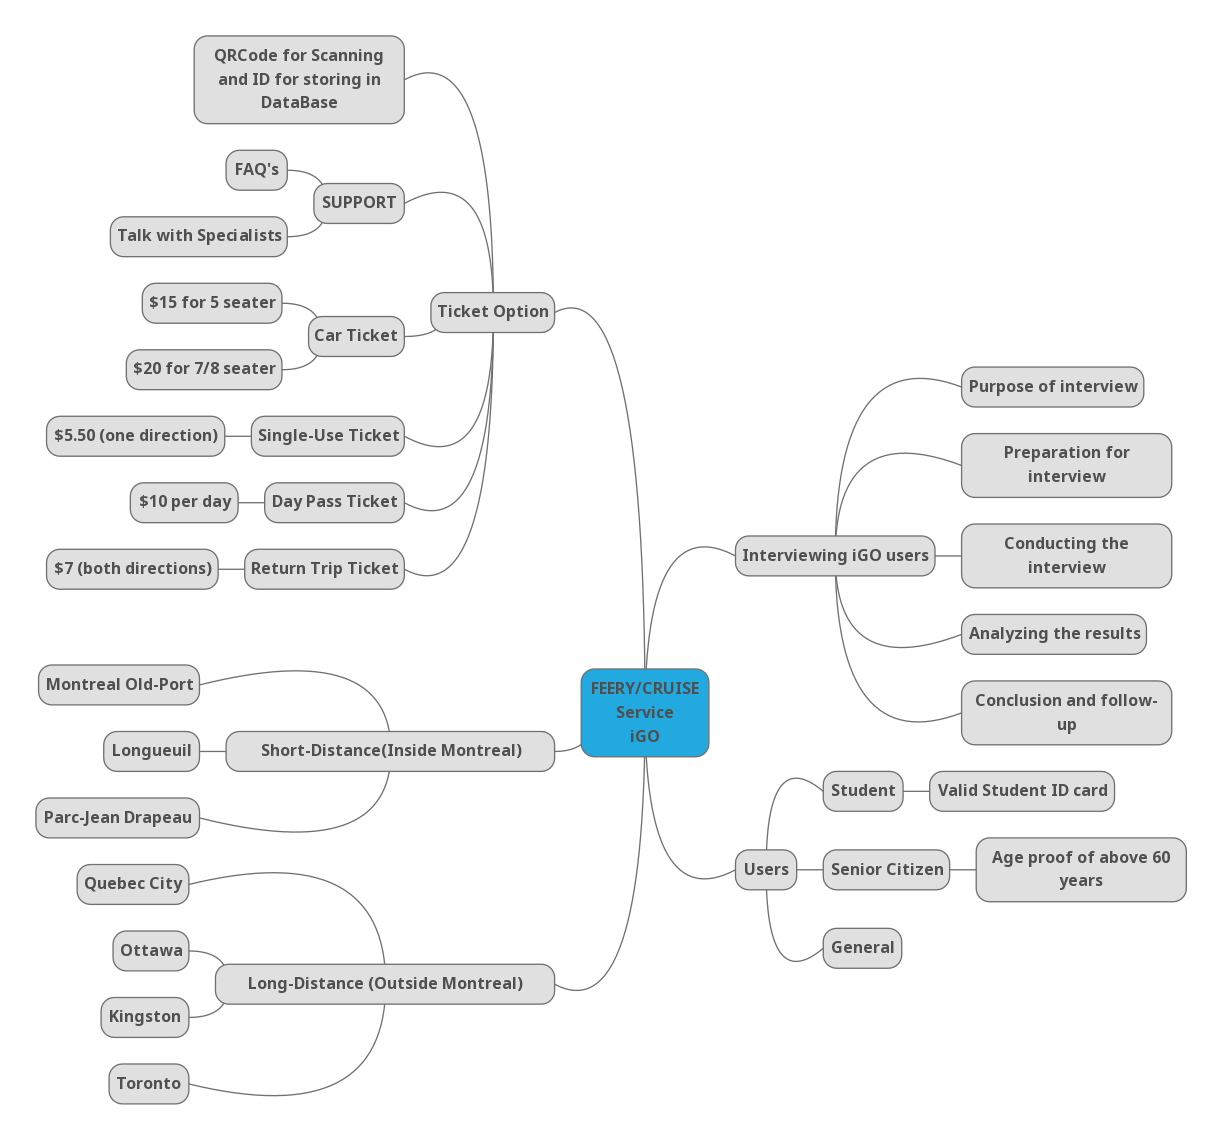
\includegraphics[height=0.52\textheight]{Interviews/MindMap/Mind Map.png}
    \caption{A mind map used for context and iGO ticket vending machine interview planning.}
    \label{fig:MindMap}
\end{figure}
\clearpage

\section{Interviews:}
Interviews were conducted on individuals we thought would reflect our customer base. The following are our succinct conclusions from each interview conducted. The first interview acts as a pilot interview. For the recorded transcript of each interview, see Appendix \ref{sec:Appendix_Interviews}.\\
Some conclusions made use of user experience principles \cite{UIgoals} as part of theory from SOEN 357.
\subsection{Interview 1}
Some of our customers may be averse to technology, and be more materialistic, preferring physical tokens and interactions over virtual ones. A skeuomorphic user interface may please customers that share similar values as this interviewee better by being grounded closer to traditional solutions, rather than the more abstract and minimalist flat design. 

However, it's also a reality that skeuomorphism takes more effort to design around and still be visually pleasant than flat design by virtue of the level in detail. 

\subsection{Interview 2}
The interface should be simple and minimalistic and require few interactions on the Commuter's part. An interface in flat design will reduce the amount of noise and make it clear what are interactable elements. There can be a little bit more emphasis on the option for choosing recreational ticket, since there's some demand for it. Purchases in advance further than a day may not be needed. Some of our customers may be inclined to technology, preferring payments through mobile apps and keeping transaction records/receipts viewable electronically. 
Some usability goals our interface should respect:
\begin{itemize}
    \item Learnability: The interface should be simple and visible enough to be easily and quickly learned how to operate. Immediate feedback would help reinforce. Virtual affordance and unambiguous design can help the Commuter intuitively know what and which purposes serve what and which actions.
    \item Efficiency usability goal: Tasks should be completable by the Commuter in as few actions as possible.
\end{itemize}

\subsection{Interview 3}
In conclusion, the interviewee shared positive feedback about the Greater Montreal Ferry System, highlighting the accessibility of the service and convenient location of terminals. They expressed interest in the recreational ticket option and appreciated the convenience of QR code ticket entry. They emphasized the importance of friendly and helpful customer service, a variety of ticket options, and year-round service availability. These salient features can provide insight for improving the overall customer experience and satisfaction with the ferry/cruise service.

\newpage
\subsection{Interview 4}
Based on the interview, the following can be concluded. The interviewee thinks that a TVM for public transportation should have features such as route information, variety of ticket options, contactless payment option, and real-time updates of the transport schedule. They believe that vending machines are an modern alternative to the traditional standing in queue for purchasing a ticket system. The interviewee also prefers a vending machine that offers both cash and card payment modes and also a variety of ticket options (e.g. single-use, day pass, or monthly pass). Additionally, they believe that security measures such as security cameras and anti-theft alarms should be included for ensuring security of both commuters and the TVM. Overall, the interviewee believes that a dynamic vending machine that can be used for multiple services would be preferable, and having a clear and easy-to-understand pricing structure for tickets is important.

\section{Conclusion}
The interviews conducted for the design of the iGo ticket vending machine provided valuable insights into the needs and preferences of commuters. By understanding the commuter's perspective, the iGo TVM can be designed to be more user-friendly and efficient, making the ticket purchasing process a more enjoyable experience for commuters.
\vspace{\baselineskip}

One key finding from the interviews was the importance of clear and concise instructions. Commuters expressed frustration when the instructions were difficult to understand or unclear. As a result, the design team made sure to prioritize the clarity of the instructions and ensured fewer steps to purchase a ticket from the start. Additionally, the design team discovered that having a way to call on-site support agents to provide assistance when needed was a valuable feature for commuters. This led to the inclusion of a "seek assistance" use case in the design.
\vspace{\baselineskip}

Another important insight gained from the interviews was the importance of multiple language options. As Montreal is a diverse city, many commuters have a first language other than English or French. Therefore, including multiple language options was seen as an essential feature for the iGo TVM.
\vspace{\baselineskip}

Furthermore, the design team learned that providing a variety of payment options was important. While some commuters preferred to pay by cash, others preferred to pay using their contact-less credit or debit card. As a result, the design team included use cases for both payment options in the design.
\vspace{\baselineskip}

In conclusion, the interviews conducted for the design of the iGo ticket vending machine provided valuable insights that helped inform the design process. By prioritizing clear instructions, including support agents for assistance, offering multiple language options, and providing a variety of payment options, the iGo TVM was designed to be a user-friendly and efficient ticket purchasing experience for commuters.

\chapter{Problem 4 : Use Case Model}
\section{Introduction}
 A use case model is a high-level view of the functionalities that a system provides to its users. It is a way to understand the requirements of the system and how users will interact with it. By creating a use case model, the developers and stakeholders of the iGo TVM can gain a better understanding of the system requirements and how the system will be used. This can help to identify potential issues or improvements before the system is implemented, ultimately leading to a more efficient and effective system.

 \section{Use case Model}
The iGo TVM Use Case diagram is a visual representation of the various interactions between the Commuter and the system during the process of purchasing a ferry ticket. The diagram shows how the Commuter can choose their desired destination, select the type of ticket, choose seats, and make a payment using either cash or a card. The iGo Ticketing Server and Bank actors are involved in processing the payments, while the Support Agent actor is available to provide assistance if needed.

This use case diagram was created using Visual Paradigm, a software development tool that enables users to create visual representations of system architectures and designs. 
The following subsections describe the Actors, abstract use case packages and the use cases given in the use case diagram:

\subsubsection{System and Actors}
\begin{itemize}
    \item Commuter: the one using our system and our primary intended recipient.
    \item iGo Ticketing Server: our system that primarily supports the operations of the Commuter.
    \item Bank: an established monetary funds handler. Card payments will be processed by this actor.
    \item Support Agent: an iGo associate, who will be able to assist a Commuter in operating iGo's TVM when asked. 
\end{itemize}

\subsection{Use Case Summaries}
\begin{enumerate}[label=UC-\arabic*]
    \item Read Instructions: The Commuter can read the instructions provided by the system to understand how to use the iGo TVM Ticketing process.
    \item Seek Assistance: The Commuter can seek assistance from the Support Agent on-site if they encounter any issues with the system.
    \item Choose Language: The Commuter can choose the language they prefer for the system's interface.
     \item Purchase Montreal Ferry Ticket: This use case helps the commuter initiate the process of booking a ticket for the Montreal ferry.
    \item Purchase Inter-City Ferry Ticket: The Commuter can initiate the process of purchase a ticket for an inter-city ferry travel.
    \item Choose Destination: The Commuter can choose their destination.
    \item Pick from Ferry Schedule: The Commuter can pick a ferry schedule.
    \item Select Ticket Type: The Commuter can select the type of ticket they want to purchase.
    \item Provide Ticket Details and Pricing: The system provides the Commuter with the details and pricing for the selected ticket.
    \item Choose Seats: The Commuter can choose the seats they prefer.
    \item Pay by Cash: The Commuter can choose to pay for their ticket using cash.
    \item Verify Cash Payment: The system verifies the cash payment made by the Commuter.
    \item Insert Cash: The Commuter can insert the cash they want to use for payment.
    \item Select Quantity: The Commuter can select the quantity of tickets they want to purchase.
    \item Pay By Card: The Commuter can choose to pay for their ticket using a card.
    \item Insert Card: The Commuter can insert their card for payment.
    \item Authenticate by PIN: The Commuter can authenticate their card payment using a PIN.
    \item Provide Ferry Timings and Availability: The system provides the Commuter with information on ferry timings and availability.
    \item Confirm Purchase: The Commuter can confirm their ticket purchase.
    \item Make a Payment: The Commuter can make a payment for their ticket.
    \item Show Payment Error: The system displays an error message if there is an issue with the payment.
    \item Display Ticket: The system displays the purchased ticket.
    \item Print Ticket: The Commuter can print their ticket.
    \item Return Cash Difference: The system returns any cash difference to the Commuter.
    \item Confirm Payment: The system confirms the payment made by the Commuter.
    \item Return Card: The system returns the Commuter's card after payment.
     \item End Session: The Commuter can end the current session with the system.
    \item Display Session End Message: The system displays a message when a session is about to end.
\end{enumerate}

\begin{figure}[ht]
    \centering
    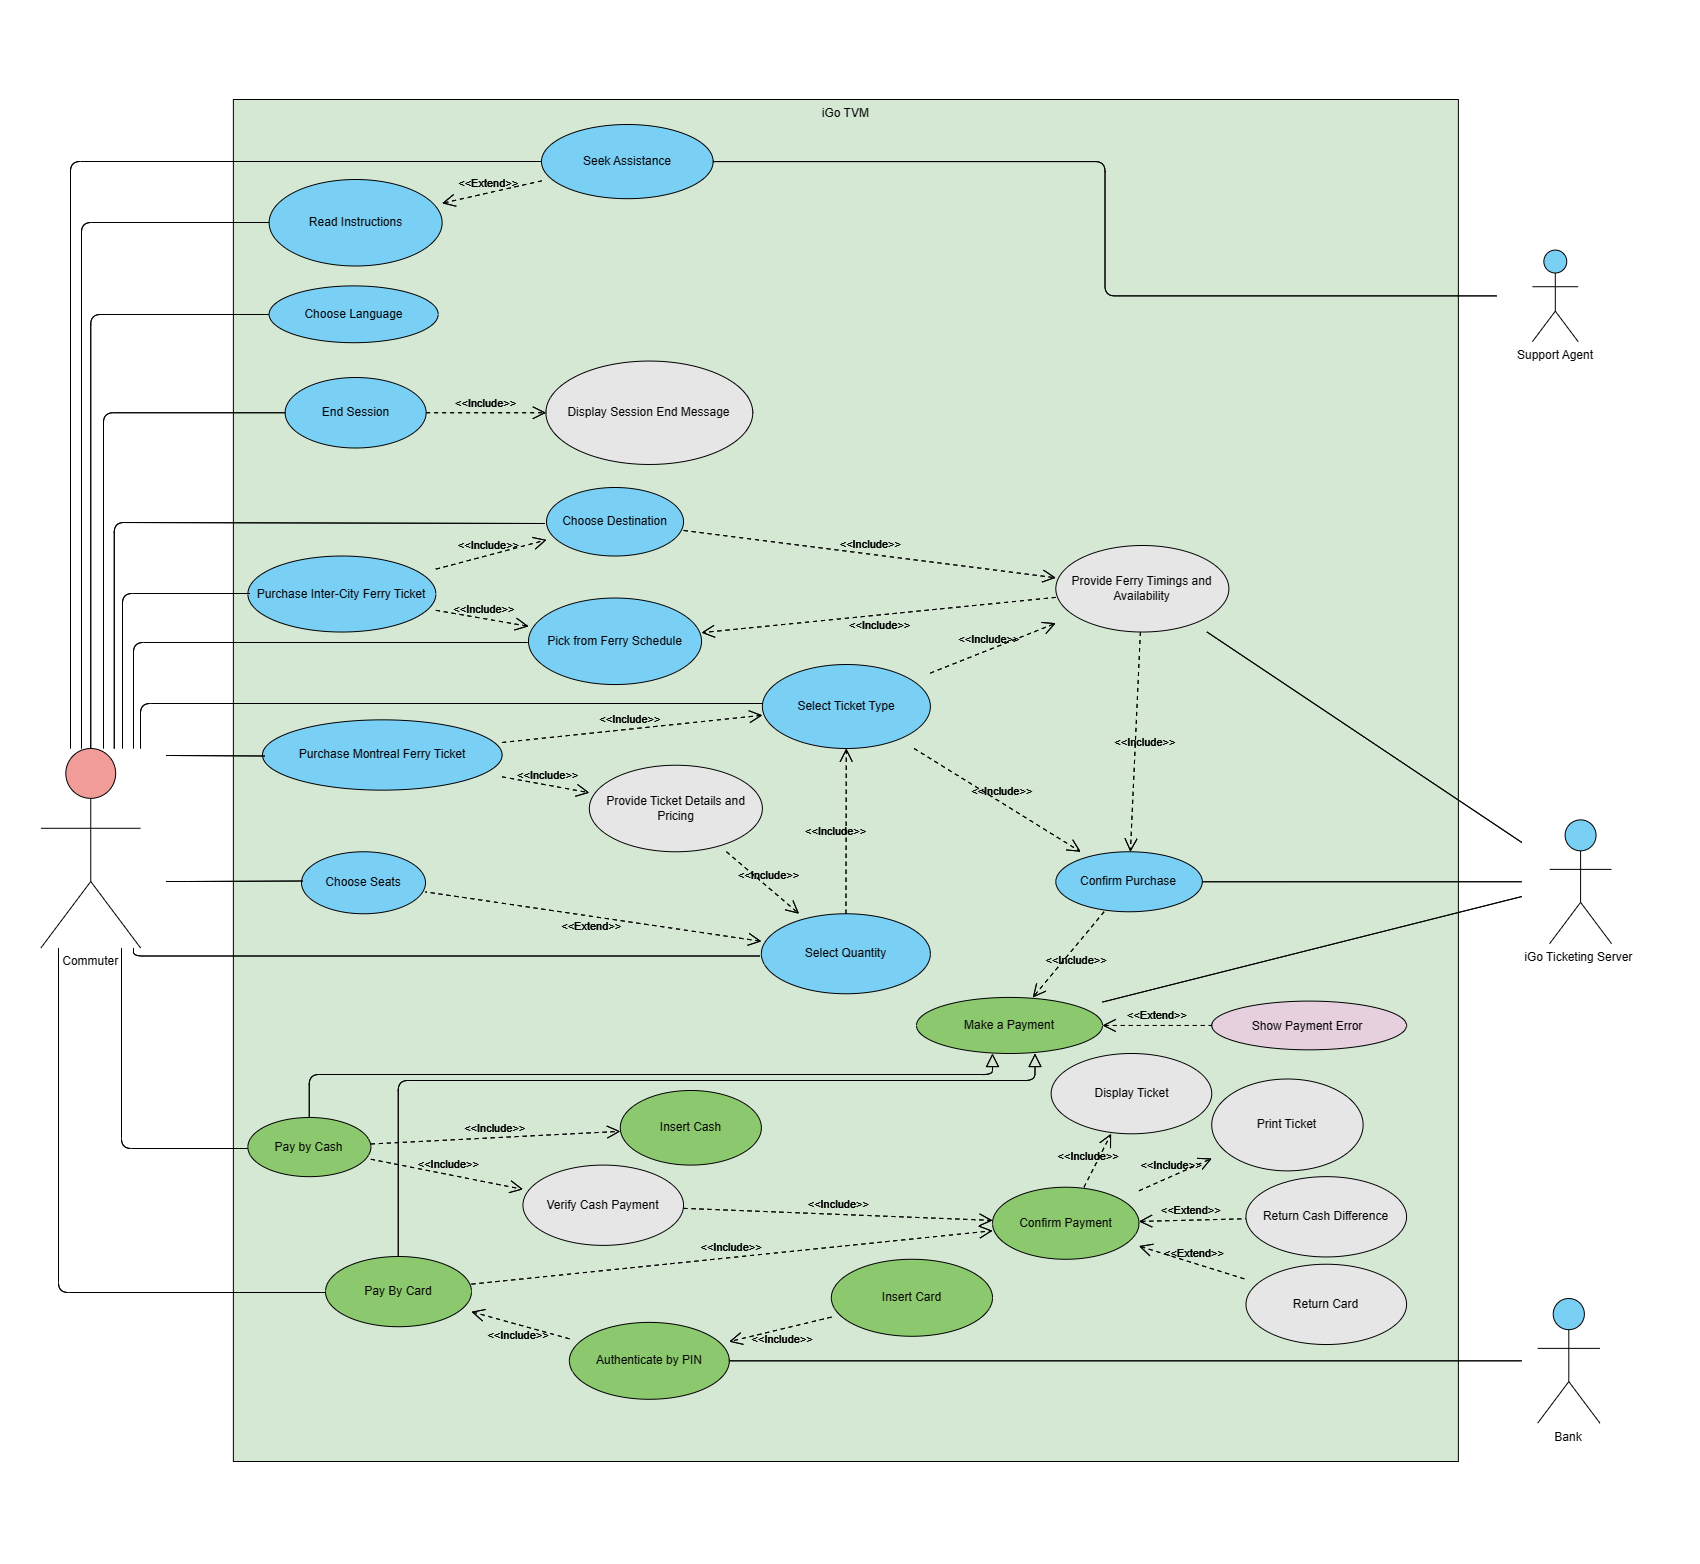
\includegraphics[width=\textwidth, height=\textheight, keepaspectratio]{UseCaseDiagrams/iGousecase.png}
    \caption{Use Case Diagram for iGo}
    \label{fig:UseCaseDiagram}
\end{figure}

\subsubsection{Use Case Categories from the use case diagram :}
The figures were created using lecture slides by Pankaj Kamthan\cite{UseCaseDiagramming} as a guide.
The use cases in Figure \ref{fig:UseCaseDiagram} are color-coded into 4 categories:
\begin{enumerate}
    \item Blue : Use cases that directly interact with the primary actor(Commuter) like selecting a destination, choosing seats, and paying for a ticket, whether by cash or card. These use cases describe the actions taken by the commuter when using the iGo TVM system.
    \item Grey : Use Cases that imply operations performed by the iGo TVM that interacts with the above use cases. Examples of these are displaying ferry schedules, Display Ticket and Print Ticket
    \item Green : Transaction Use cases - These use cases are involved with the payment systems in the iGo TVM like Make a Payment, Pay by Cash, Pay by Card and Confirm Payment
    \item Red :  This represents an error notification by the iGo TVM system. In this case it is used in the Show Payment Error use case.
\end{enumerate}

\begin{figure}
    \centering
    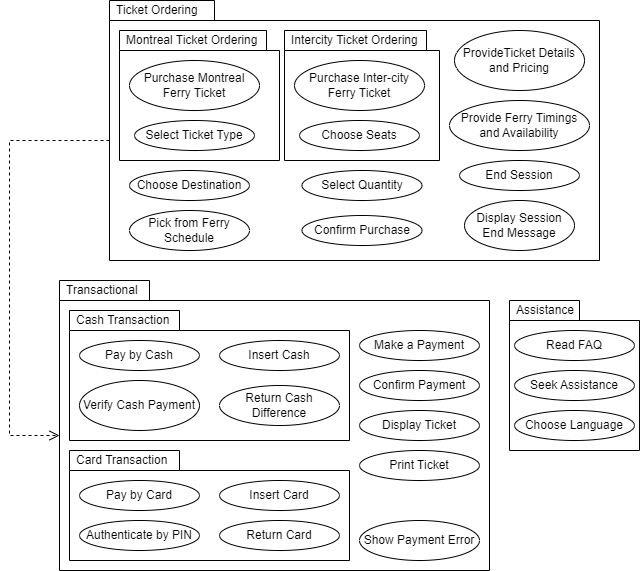
\includegraphics[width=\textwidth]{UseCaseDiagrams/Package Diagram of Use Cases.png}
    \caption{Package Diagram of Use Cases}
    \label{fig:UseCasePackage}
\end{figure}

\section{Use Case Packages}
The package diagram in figure \ref{fig:UseCasePackage} for the iGo TVM has divided the use cases into three distinct top-level packages: 
\begin{enumerate}
\item Ticket Ordering : The first package is called Ticket Ordering and contains use cases that describe the process of ordering a ticket from the vending machine. These use cases include selecting a destination, picking from ferry schedules, selecting ticket type, choosing seats, and displaying and printing tickets. 
There are 2 sub-packages in this Package : 
\begin{enumerate}
    \item Montreal Ticket ordering : use cases pertaining to only Montreal ferry Booking
    \item Intercity Ticket ordering : use cases pertaining to only Intercity ferry Booking
\end{enumerate}

\item Transactional : The second package is called Transactional and includes all the use cases related to payment processing. These use cases include making a payment, paying by cash or card, verifying cash payment, inserting cash, inserting a card for payment, authenticating the card payment with a PIN, returning cash difference, confirming payment, and returning the commuter's card after payment.
There are 2 sub-packages in this package 
\begin{enumerate}
    \item Cash Transaction : use cases pertaining to cash based transactions
    \item Card Transaction : use cases pertaining to bank card(credit/debit and contact-less) based transactions
\end{enumerate}

\item Assistance : The third package is called Assistance, and it provides use cases related to supporting commuters who encounter issues with the system. These use cases include reading instructions and seeking assistance from support agents.

By dividing the use cases into these three packages, the diagram helps to simplify the understanding of the iGo ticket vending machine system by showing how the different use cases are related to each other and how they interact with the commuter and the vending machine. It also highlights the importance of the payment processing system and the need for assistance to ensure a seamless experience for the commuter.
\end{enumerate}

\section{Use Case Definitions}

%\begin{enumerate*}[itemjoin=\newline] creates a typical numbered list, but does not start with a linebreak.
\begin{table}[ht]
    \centering
    \begin{tabular}{|l|p{11cm}|}
         \hline
         System             & iGo\\
         \hline
         Identifier         & UC-1 \\
         \hline
         Name               & Read Instructions \\
         \hline
         Pre-Condition(s)   & 
         \begin{enumerate*}[itemjoin=\newline]
             \item Commuter is at the terminal.
         \end{enumerate*} \\
         \hline
         Post-Condition(s)  & 
         \begin{enumerate*}[itemjoin=\newline]
             \item Instructions for that specific page is displayed 
         \end{enumerate*} \\
         \hline
         Trigger            & Commuter clicks the help option on any screen \\
         \hline
         Normal Flow        & 
         \begin{enumerate*}[itemjoin=\newline]
             \item Once the help button is clicked, it shows instructions based on the page it is in.
             % \item The commuter can then choose to request on-site booking support from an on-site support agent.
         \end{enumerate*} \\
         \hline
         Exceptional Flow(s)& None\\
         \hline
         Related Actor(s)   & Commuter \\
         \hline
         Related Use Case(s)& Seek Assistance\\
         \hline
    \end{tabular}
    \caption{Use Case for Read Instructions}
    \label{tab:UC_ReadInstructions}
\end{table}

\begin{table}[ht]
    \centering
    \begin{tabular}{|l|p{11cm}|}
         \hline
         System             & iGo\\
         \hline
         Identifier         & UC-2 \\
         \hline
         Name               & Seek Assistance \\
         \hline
         Pre-Condition(s)   & 
         \begin{enumerate*}[itemjoin=\newline]
             \item Commuter is in the Read Instructions Page.
         \end{enumerate*} \\
         \hline
         Post-Condition(s)  & 
         \begin{enumerate*}[itemjoin=\newline]
             \item A signal is sent to the terminal to a support agent to come and assist the commuter.
         \end{enumerate*} \\
         \hline
         Trigger            & Commuter clicks the seek Assistance button \\
         \hline
         Normal Flow        & 
         \begin{enumerate*}[itemjoin=\newline]
             \item As soon as the seek assistance button in the instructions page is clicked, the terminal support agent is notified to assist the commuter
         \end{enumerate*} \\
         \hline
         Exceptional Flow(s)& None\\
         \hline
         Related Actor(s)   & Commuter, Support Agent \\
         \hline
         Related Use Case(s)& Read Instructions\\
         \hline
    \end{tabular}
    \caption{Use Case for Seek Assistance}
    \label{tab:UC_SeekAssistance}
\end{table}

\begin{table}[ht]
    \centering
    \begin{tabular}{|l|p{11cm}|}
         \hline
         System             & iGo\\
         \hline
         Identifier         & UC-3 \\
         \hline
         Name               & Choose Language \\
         \hline
         Pre-Condition(s)   & 
         \begin{enumerate*}[itemjoin=\newline]
             \item Commuter is at the terminal.
         \end{enumerate*} \\
         \hline
         Post-Condition(s)  & 
         \begin{enumerate*}[itemjoin=\newline]
             \item Interface language is set to the Commuter's preference.
             \item Commuter is able to understand the language of the interface.
         \end{enumerate*} \\
         \hline
         Trigger            & Commuter clicks the change Language button \\
         \hline
         Normal Flow        & 
         \begin{enumerate*}[itemjoin=\newline]
             \item The terminal shows language options for English and French.
             \item The Commuter selects his preferred language.
         \end{enumerate*} \\
         \hline
         Exceptional Flow(s)& 
         \begin{enumerate*}[itemjoin=\newline]
             \item Commuter aborts choosing a language.
         \end{enumerate*} \\
         \hline
         Related Actor(s)   & Commuter \\
         \hline
         Related Use Case(s)& None\\
         \hline
    \end{tabular}
    \caption{Use Case for Choose Language}
    \label{tab:UC_ChooseLanguage}
\end{table}

\begin{table}[ht]
    \centering
    \begin{tabular}{|l|p{11cm}|}
         \hline
         System             & iGo\\
         \hline
         Identifier         & UC-4 \\
         \hline
         Name               & Purchase Montreal Ferry Ticket \\
         \hline
         Pre-Condition(s)   & 
         \begin{enumerate*}[itemjoin=\newline]
             \item Commuter Selected the language
         \end{enumerate*} \\
         \hline
         Post-Condition(s)  & 
         \begin{enumerate*}[itemjoin=\newline]
            \item Commuter is in possession of an Montreal ferry ticket. 
         \end{enumerate*} \\
         \hline
         Trigger            & Commuter selects the Montreal Ferry ticket choice. \\
         \hline
         Normal Flow        & 
         \begin{enumerate*}[itemjoin=\newline]
           \item Commuter picks a ticket type according to UC-8.
            \item Commuter picks a quantity of tickets according to UC-14.
            \item Commuter confirms his purchase according to UC-19.
            \item Commuter pays the ticket by his preferred method.
            \item Commuter receives his ticket.
         \end{enumerate*} \\
         \hline
         Exceptional Flow(s)& 
         \begin{enumerate*}[itemjoin=\newline]
             \item Anytime, the Commuter aborts the purchase.
         \end{enumerate*} \\
         \hline
         Related Actor(s)   & Commuter \\
         \hline
         Related Use Case(s)& Select Ticket Type\\
         \hline
    \end{tabular}
    \caption{Use Case for Purchase Montreal Ferry Ticket}
    \label{tab:UC_PurchaseMontrealFerryTicket}
\end{table}

\begin{table}[ht]
    \centering
    \begin{tabular}{|l|p{11cm}|}
         \hline
         System             & iGo\\
         \hline
         Identifier         & UC-5 \\
         \hline
         Name               & Purchase Inter-City Ferry Ticket \\
         \hline
         Pre-Condition(s)   & 
         \begin{enumerate*}[itemjoin=\newline]
             \item Commuter is at the terminal.
         \end{enumerate*} \\
         \hline
         Post-Condition(s)  & 
         \begin{enumerate*}[itemjoin=\newline]
            \item Commuter is in possession of an inter-city ferry ticket. 
         \end{enumerate*} \\
         \hline
         Trigger            & Commuter selects the intercity ticket choice. \\
         \hline
         Normal Flow        & 
         \begin{enumerate*}[itemjoin=\newline]
            \item Commuter picks a destination according to UC-6.
            \item The Terminal displays the ferry schedules according to UC-18.
            \item Commuter picks a ferry from a schedule according to UC-7.
            \item The Terminal displays ticket choices according to UC-9.
            \item Commuter picks a quantity of tickets according to UC-14.
            \item Commuter chooses which seats to reserve with the ticket according to UC-10.
            \item Commuter confirms his purchase according to UC-19.
            \item Commuter pays the ticket by his preferred method.
            \item Commuter receives his ticket.
         \end{enumerate*} \\
         \hline
         Exceptional Flow(s)& 
         \begin{enumerate*}[itemjoin=\newline]
             \item Anytime, the Commuter aborts the purchase.
         \end{enumerate*} \\
         \hline
         Related Actor(s)   & Commuter, iGo System \\
         \hline
         Related Use Case(s)& UC-6, UC-7, UC-9, UC-10, UC-11, UC-15, UC-22, UC-23, UC-25\\
         \hline
    \end{tabular}
    \caption{Use Case for Purchase Inter-City Ferry Ticket}
    \label{tab:UC_PurchaseInterCityFerryTicket}
\end{table}

\begin{table}[ht]
    \centering
    \begin{tabular}{|l|p{11cm}|}
         \hline
         System             & iGo\\
         \hline
         Identifier         & UC-6 \\
         \hline
         Name               & Choose Destination \\
         \hline
         Pre-Condition(s)   & 
         \begin{enumerate*}[itemjoin=\newline]
             \item Commuter is at the terminal.
             \item Commuter is ordering a ticket.
         \end{enumerate*} \\
         \hline
         Post-Condition(s)  & 
         \begin{enumerate*}[itemjoin=\newline]
             \item Commuter's ticket's destination is determined.
         \end{enumerate*} \\
         \hline
         Trigger            & Commuter is prompted to choose a destination by the terminal. \\
         \hline
         Normal Flow        & 
         \begin{enumerate*}[itemjoin=\newline]
             \item The Commuter selects his intended destination
         \end{enumerate*} \\
         \hline
         Exceptional Flow(s)& 
         \begin{enumerate*}[itemjoin=\newline]
             \item Commuter aborts choosing a destination.
         \end{enumerate*} \\
         \hline
         Related Actor(s)   & Commuter \\
         \hline
         Related Use Case(s)& UC-4, UC-5\\
         \hline
    \end{tabular}
    \caption{Use Case for Choose Destination}
    \label{tab:UC_ChooseDestination}
\end{table}


\begin{table}[ht]
    \centering
    \begin{tabular}{|l|p{11cm}|}
        \hline
        System             & iGo\\
        \hline
        Identifier         & UC-7 \\
        \hline
        Name               & Pick from Ferry Schedule \\
        \hline
        Pre-Condition(s)   & 
        \begin{enumerate*}[itemjoin=\newline]
            \item Commuter is at the terminal.
            \item Commuter is ordering a ticket.
            \item Commuter has selected a destination.
        \end{enumerate*} \\
        \hline
        Post-Condition(s)  & 
        \begin{enumerate*}[itemjoin=\newline]
            \item Commuter's ticket's schedule is determined.
        \end{enumerate*} \\
        \hline
        Trigger            & Commuter is prompted to choose a ferry from a list of schedules by the terminal. \\
        \hline
        Normal Flow        & 
        \begin{enumerate*}[itemjoin=\newline]
            \item The terminal displays ferries by their schedules for the given destination according to UC-18.
            \item The Commuter selects his preferred schedule for the ticket.
        \end{enumerate*} \\
        \hline
        Exceptional Flow(s)& 
        \begin{enumerate*}[itemjoin=\newline]
            \item Commuter aborts choosing a schedule.
        \end{enumerate*} \\
        \hline
        Related Actor(s)   & Commuter \\
        \hline
        Related Use Case(s)& UC-4, UC-5, UC-18\\
        \hline
    \end{tabular}
    \caption{Use Case for Pick from Ferry Schedule}
    \label{tab:UC_PickFromFerrySchedule}
\end{table}

\begin{table}[ht]
    \centering
    \begin{tabular}{|l|p{11cm}|}
        \hline
        System             & iGo\\
        \hline
        Identifier         & UC-8 \\
        \hline
        Name               & Select Ticket Type \\
        \hline
        Pre-Condition(s)   & 
        \begin{enumerate*}[itemjoin=\newline]
            \item Commuter is at the terminal.
            \item Commuter is ordering a Montreal ferry ticket.
        \end{enumerate*} \\
        \hline
        Post-Condition(s)  & 
        \begin{enumerate*}[itemjoin=\newline]
            \item Commuter's Montreal ferry ticket's type is determined
        \end{enumerate*} \\
        \hline
        Trigger            & Commuter is prompted to choose a ticket type by the terminal. \\
        \hline
        Normal Flow        & 
        \begin{enumerate*}[itemjoin=\newline]
            \item The terminal displays details of the Commuter's ticket choices according to UC-9.
            \item The Commuter selects his preferred ticket type.
        \end{enumerate*} \\
        \hline
        Exceptional Flow(s)& 
        \begin{enumerate*}[itemjoin=\newline]
            \item Commuter aborts choosing a ticket type.
        \end{enumerate*} \\
        \hline
        Related Actor(s)   & Commuter \\
        \hline
        Related Use Case(s)& UC-4, UC-9\\
        \hline
    \end{tabular}
    \caption{Use Case for Select Ticket Type}
    \label{tab:UC_SelectTicketType}
\end{table}

\begin{table}[ht]
    \centering
    \begin{tabular}{|l|p{11cm}|}
        \hline
        System             & iGo\\
        \hline
        Identifier         & UC-9 \\
        \hline
        Name               & Provide Ticket Details and Pricing \\
        \hline
        Pre-Condition(s)   & 
        \begin{enumerate*}[itemjoin=\newline]
            \item Commuter is at the terminal.
        \end{enumerate*} \\
        \hline
        Post-Condition(s)  & 
        \begin{enumerate*}[itemjoin=\newline]
            \item Commuter is knowledgeable on tickets and their prices.
        \end{enumerate*} \\
        \hline
        Trigger            & The terminal wants to ensure the Commuter knows about tickets. \\
        \hline
        Normal Flow        & 
        \begin{enumerate*}[itemjoin=\newline]
            \item If the Commuter is currently ordering a Montreal ferry ticket, the terminal displays descriptions and pricing of the different options he has.
            \item Otherwise, the terminal displays the pricing of intercity tickets.
        \end{enumerate*} \\
        \hline
        Exceptional Flow(s)& None\\
        \hline
        Related Actor(s)   & iGo System \\
        \hline
        Related Use Case(s)& UC-4, UC-5\\
        \hline
    \end{tabular}
    \caption{Use Case for Provide Ticket Details and Pricing}
    \label{tab:UC_ProvideTicketDetailsAndPricing}
\end{table}

\begin{table}[ht]
    \centering
    \begin{tabular}{|l|p{11cm}|}
        \hline
        System             & iGo\\
        \hline
        Identifier         & UC-10 \\
        \hline
        Name               & Choose Seats \\
        \hline
        Pre-Condition(s)   & 
        \begin{enumerate*}[itemjoin=\newline]
            \item Commuter is at the terminal.
            \item Commuter is ordering an intercity ferry ticket.
            \item Commuter has chosen a ferry.
            \item Commuter has chosen his number of tickets.
        \end{enumerate*} \\
        \hline
        Post-Condition(s)  & 
        \begin{enumerate*}[itemjoin=\newline]
            \item Commuter's preferred seats are determined. 
        \end{enumerate*} \\
        \hline
        Trigger            & Commuter is prompted to choose his seats by the terminal. \\
        \hline
        Normal Flow        & 
        \begin{enumerate*}[itemjoin=\newline]
            \item The terminal offers the Commuter a selection of seats.
            \item The Commuter selects his preferred seats, as many as he has tickets ordered.
            \item OR, the Commuter allows iGo system to determine his seats in his place.
        \end{enumerate*} \\
        \hline
        Exceptional Flow(s)& 
        \begin{enumerate*}[itemjoin=\newline]
            \item Commuter aborts choosing a ticket type.
        \end{enumerate*} \\
        \hline
        Related Actor(s)   & Commuter, iGo System \\
        \hline
        Related Use Case(s)& UC-5, UC-14\\
        \hline
    \end{tabular}
    \caption{Use Case for Choose Seats}
    \label{tab:UC_ChooseSeats}
\end{table}

\begin{table}[ht]
    \centering
    \begin{tabular}{|l|p{11cm}|}
        \hline
        System             & iGo\\
        \hline
        Identifier         & UC-11 \\
        \hline
        Name               & Pay By Cash \\
        \hline
        Pre-Condition(s)   & 
        \begin{enumerate*}[itemjoin=\newline]
            \item Commuter has confirmed the purchase and selected the payment option
        \end{enumerate*} \\
        \hline
        Post-Condition(s)  & 
        \begin{enumerate*}[itemjoin=\newline]
            \item Commuter gets payment confirmed notification and gets his ticket
        \end{enumerate*} \\
        \hline
        Trigger            & Payment option to pay be cash is selected \\
        \hline
        Normal Flow        & 
        \begin{enumerate*}[itemjoin=\newline]
            \item Once the payment by cash is selected, the commuter enters the cash into the machine (UC-13)
            \item The machine processes the payment and returns the cash difference(UC-24)
            \item After this the commuter recieves his ticket
        \end{enumerate*} \\
        \hline
        Exceptional Flow(s)& Commuter didnt enter the cash or cancelled the session(UC-27)\\
        \hline
        Related Actor(s)   & iGo System \\
        \hline
        Related Use Case(s)& UC-4, UC-5\\
        \hline
    \end{tabular}
    \caption{Use Case for Pay By Cash}
    \label{tab:UC_PayByCash}
\end{table}

\begin{table}[ht]
    \centering
    \begin{tabular}{|l|p{11cm}|}
        \hline
        System             & iGo\\
        \hline
        Identifier         & UC-12 \\
        \hline
        Name               & Verify Cash Payment \\
        \hline
        Pre-Condition(s)   & None \\
        \hline
        Post-Condition(s)  & 
        \begin{enumerate*}[itemjoin=\newline]
            \item Commuter's excess cash is reimbursed.
        \end{enumerate*} \\
        \hline
        Trigger            & Commuter handed cash to the terminal. \\
        \hline
        Normal Flow        & 
        \begin{enumerate*}[itemjoin=\newline]
            \item The terminal calculates the difference between expected and actual payment by the Commuter.
            \item The terminal reimburses the Commuter for his excess cash payment.
        \end{enumerate*} \\
        \hline
        Exceptional Flow(s)& 
        \begin{enumerate*}[itemjoin=\newline]
            \item Commuter pays too little, then ask for more cash.
            \item Commuter cancels payment, then reimburse total cash inputted by the Commuter.
        \end{enumerate*} \\
        \hline
        Related Actor(s)   & Commuter\\
        \hline
        Related Use Case(s)& UC-4, UC-5, UC-13\\
        \hline
    \end{tabular}
    \caption{Use Case for Verify Cash Payment}
    \label{tab:UC_VerifyCashPayment}
\end{table}

\begin{table}[ht]
    \centering
    \begin{tabular}{|l|p{11cm}|}
        \hline
        System             & iGo\\
        \hline
        Identifier         & UC-13 \\
        \hline
        Name               & Insert Cash \\
        \hline
        Pre-Condition(s)   & 
        \begin{enumerate*}[itemjoin=\newline]
            \item Commuter has selected the pay by cash option
        \end{enumerate*} \\
        \hline
        Post-Condition(s)  & 
        \begin{enumerate*}[itemjoin=\newline]
            \item The cash is calculated, difference is returned and the ticket is printed
        \end{enumerate*} \\
        \hline
        Trigger            & option to pay be cash is selected and user enters the cash \\
        \hline
        Normal Flow        & 
        \begin{enumerate*}[itemjoin=\newline]
            \item Once the payment by cash is selected, the commuter enters the cash into the machine
            \item The machine processes the payment and returns the cash difference(UC-24)
            \item After this the commuter receives his ticket(UC-22, UC-23)
        \end{enumerate*} \\
        \hline
        Exceptional Flow(s)& Commuter didn't enter the cash or cancelled the session(UC-27)\\
        \hline
        Related Actor(s)   & Commuter\\
        \hline
        Related Use Case(s)& UC-11, UC-12,UC-24\\
        \hline
    \end{tabular}
    \caption{Use Case for Insert Cash}
    \label{tab:UC_InsertCash}
\end{table}
\begin{table}[ht]
    \centering
    \begin{tabular}{|l|p{11cm}|}
        \hline
        System             & iGo\\
        \hline
        Identifier         & UC-14 \\
        \hline
        Name               & Select Quantity \\
        \hline
        Pre-Condition(s)   & 
        \begin{enumerate*}[itemjoin=\newline]
            \item Commuter has selected the type of ticket
        \end{enumerate*} \\
        \hline
        Post-Condition(s)  & 
        \begin{enumerate*}[itemjoin=\newline]
            \item omce quantity is selected, it goes to the payment confirmation stage
        \end{enumerate*} \\
        \hline
        Trigger            & Type of ticket is selected \\
        \hline
        Normal Flow        & 
        \begin{enumerate*}[itemjoin=\newline]
            \item Once Type of ticket is selected, the quantity page appears
            \item Once the quantity is selected, the system provides the confirmation of booking to continue to payment(UC-19)
        \end{enumerate*} \\
        \hline
        Exceptional Flow(s)& Commuter cancelles the session(UC-27)\\
        \hline
        Related Actor(s)   & Commuter\\
        \hline
        Related Use Case(s)& UC-8, UC-19,UC-20\\
        \hline
    \end{tabular}
    \caption{Use Case for Select Quantity}
    \label{tab:UC_Select Quantity Cash}
\end{table}
\begin{table}[ht]
    \centering
    \begin{tabular}{|l|p{11cm}|}
        \hline
        System             & iGo\\
        \hline
        Identifier         & UC-15 \\
        \hline
        Name               & Pay By Card \\
        \hline
        Pre-Condition(s)   & 
        \begin{enumerate*}[itemjoin=\newline]
            \item Commuter has confirmed the purchase and selected the payment option
        \end{enumerate*} \\
        \hline
        Post-Condition(s)  & 
        \begin{enumerate*}[itemjoin=\newline]
            \item Commuter gets payment confirmed notification and gets his ticket
        \end{enumerate*} \\
        \hline
        Trigger            & Payment option to pay by Card is selected \\
        \hline
        Normal Flow        & 
        \begin{enumerate*}[itemjoin=\newline]
            \item Once the payment by Card is selected, the commuter inserts the card into the machine (UC-16)
            \item The machine requests the pin and authenticates the pin(UC-17)
            \item After this the commuter receives Confirmation
        \end{enumerate*} \\
        \hline
        Exceptional Flow(s)& Commuter didnt insert the card or cancelled the session(UC-27)\\
        \hline
        Related Actor(s)   & iGo System \\
        \hline
        Related Use Case(s)&  UC-19, UC-16\\
        \hline
    \end{tabular}
    \caption{Use Case for Pay By Card}
    \label{tab:UC_PayByCard}
\end{table}
\begin{table}[ht]
    \centering
    \begin{tabular}{|l|p{11cm}|}
        \hline
        System             & iGo\\
        \hline
        Identifier         & UC-16 \\
        \hline
        Name               & Insert Card \\
        \hline
        Pre-Condition(s)   & 
        \begin{enumerate*}[itemjoin=\newline]
            \item Commuter has confirmed the purchase and selected the pay by Card option
        \end{enumerate*} \\
        \hline
        Post-Condition(s)  & 
        \begin{enumerate*}[itemjoin=\newline]
            \item Commuter gets payment confirmed notification and gets his ticket
        \end{enumerate*} \\
        \hline
        Trigger            & Payment option to pay by Card is selected \\
        \hline
        Normal Flow        & 
        \begin{enumerate*}[itemjoin=\newline]
            \item The commuter inserts the card into the machine (UC-16)
            \item The machine requests the pin and authenticates the pin(UC-17)
            \item After this the commuter receives Confirmation
        \end{enumerate*} \\
        \hline
        Exceptional Flow(s)& Commuter didnt insert the card or cancelled the session(UC-27)\\
        \hline
        Related Actor(s)   & Commuter \\
        \hline
        Related Use Case(s)&  UC-19, UC-16\\
        \hline
    \end{tabular}
    \caption{Use Case for Insert Card}
    \label{tab:UC_InsertCard}
\end{table}
\begin{table}[ht]
    \centering
    \begin{tabular}{|l|p{11cm}|}
        \hline
        System             & iGo\\
        \hline
        Identifier         & UC-17 \\
        \hline
        Name               & Authenticate by Pin \\
        \hline
        Pre-Condition(s)   & 
        \begin{enumerate*}[itemjoin=\newline]
            \item Commuter has inserted the Bank Card and System requests Pin
        \end{enumerate*} \\
        \hline
        Post-Condition(s)  & 
        \begin{enumerate*}[itemjoin=\newline]
            \item Commuter gets payment confirmed notification and gets his ticket
        \end{enumerate*} \\
        \hline
        Trigger            & Payment option to pay by Card is selected \\
        \hline
        Normal Flow        & 
        \begin{enumerate*}[itemjoin=\newline]
            \item The machine requests the pin and authenticates the pin(UC-17)
            \item After this the commuter receives Confirmation from the System
        \end{enumerate*} \\
        \hline
        Exceptional Flow(s)& 
        \begin{enumerate*}[itemjoin=\newline]
            \item Commuter didnt enter the pin
            \item The pin is Incorrect
            \item Commuter cancelled the session(UC-27)
        \end{enumerate*} \\ or \\
        \hline
        Related Actor(s)   & Commuter \\
        \hline
        Related Use Case(s)&  UC-19, UC-16\\
        \hline
    \end{tabular}
    \caption{Use Case for Authenticate by Pin}
    \label{tab:UC_AuthenticateByPin}
\end{table}
\begin{table}[ht]
    \centering
    \begin{tabular}{|l|p{11cm}|}
        \hline
        System             & iGo\\
        \hline
        Identifier         & UC-18 \\
        \hline
        Name               & Provide Ferry Timings and Availability \\
        \hline
        Pre-Condition(s)   & 
        \begin{enumerate*}[itemjoin=\newline]
            \item Commuter has clicked the Intercity ferry Ticket option and selected the destination
        \end{enumerate*} \\
        \hline
        Post-Condition(s)  & 
        \begin{enumerate*}[itemjoin=\newline]
            \item Commuter selects ticket and continues to select quantity(UC-14)
        \end{enumerate*} \\
        \hline
        Trigger            & Commuter selects a destination in the intercity ferry option \\
        \hline
        Normal Flow        & 
        \begin{enumerate*}[itemjoin=\newline]
           \item Commuter picks a destination according to UC-6.
            \item The TVM displays the ferry schedules.
            \item Commuter picks a ferry from a schedule according to UC-7.
            \item The Terminal displays ticket choices according to UC-9.
            \item Commuter picks a quantity of tickets according to UC-14.
        \end{enumerate*} \\
        \hline
        Exceptional Flow(s) & Commuter cancelled the session(UC-27) \\
        \hline
        System   &  iGo TVM \\
        \hline
        Related Use Case(s)&  UC-6, UC-9, UC-14\\
        \hline
    \end{tabular}
    \caption{Use Case for Provide Ferry Timings and Availability}
    \label{tab:UC_ProvideFerryTimingsAvailability}
\end{table}

\begin{table}[ht]
    \centering
    \begin{tabular}{|l|p{11cm}|}
        \hline
        System             & iGo\\
        \hline
        Identifier         & UC-19 \\
        \hline
        Name               & Confirm Purchase \\
        \hline
        Pre-Condition(s)   & 
        \begin{enumerate*}[itemjoin=\newline]
            \item Commuter has selected the ticket type and quantity 
        \end{enumerate*} \\
        \hline
        Post-Condition(s)  & 
        \begin{enumerate*}[itemjoin=\newline]
            \item Commuter selects payment type and proceeds to payment
        \end{enumerate*} \\
        \hline
        Trigger            & Commuter selects the quantity (UC-14)\\
        \hline
        Normal Flow        & 
        \begin{enumerate*}[itemjoin=\newline]
            \item The Terminal displays ticket choices according to UC-9.
            \item Commuter picks a quantity of tickets according to UC-14.
            \item Commuter is prompted to confirm the purchase 
            \item Commuter proceeds to payment methods(UC-11, UC-15)
        \end{enumerate*} \\
        \hline
        Exceptional Flow(s) & Commuter cancelled the session(UC-27) \\
        \hline
         Related Actor(s)   &  Commuter \\
        \hline
        Related Use Case(s)&  UC-9, UC-14, UC-11, UC-15\\
        \hline
    \end{tabular}
    \caption{Use Case for Confirm Purchase}
    \label{tab:UC_ConfirmPurchase}
\end{table}

\begin{table}[ht]
    \centering
    \begin{tabular}{|l|p{11cm}|}
        \hline
        System             & iGo\\
        \hline
        Identifier         & UC-20 \\
        \hline
        Name               & Make a Payment \\
        Pre-Condition(s)   & 
        \begin{enumerate*}[itemjoin=\newline]
            \item Commuter has selected the ticket type and quantity 
            \item Confirm the Purchase(UC-19)
        \end{enumerate*} \\
        \hline
        Post-Condition(s)  & 
        \begin{enumerate*}[itemjoin=\newline]
            \item Commuter selects payment type(Cash or Card) and proceeds to payment
        \end{enumerate*} \\
        \hline
        Trigger            & Commuter confirms the Purchase (UC-19)\\
        \hline
        Normal Flow        & 
        \begin{enumerate*}[itemjoin=\newline]
            \item Commuter is prompted to confirm the purchase 
            \item Commuter proceeds to payment methods(Cash: UC-11, Card : UC-15)
        \end{enumerate*} \\
        \hline
        Exceptional Flow(s) & Commuter cancelled the session(UC-27) \\
        \hline
         Related Actor(s)   &  Commuter, Bank \\
        \hline
        Related Use Case(s)& UC-18, UC-11, UC-15\\
        \hline
    \end{tabular}
    \caption{Use Case for Make a Payment}
    \label{tab:UC_MakePayment}
\end{table}

\begin{table}[ht]
    \centering
    \begin{tabular}{|l|p{10cm}|}
        \hline
        System             & iGo\\
        \hline
        Identifier         & UC-21 \\
        \hline
        Name               &  Show Payment Error \\
        Pre-Condition(s)   & 
        \begin{enumerate*}[itemjoin=\newline]
            \item Commuter has Confirmed purchase (UC-19)
            \item Commuter has reached the Make a Payment Page and discarded or made an incorrect payment 
        \end{enumerate*} \\
        \hline
        Post-Condition(s)  & 
        \begin{enumerate*}[itemjoin=\newline]
            \item The Transaction gets terminated
        \end{enumerate*} \\
        \hline
        Trigger(s)            & 
         \begin{enumerate*}[itemjoin=\newline]
            \item Commuter Either ends the session(UC-27)
            \item System Rejects the Payment(Card: Bank, Cash : System)
        \end{enumerate*} \\
        \hline
        Normal Flow        & 
        \begin{enumerate*}[itemjoin=\newline]
            \item Commuter proceeds to payment methods(Cash: UC-11, Card: UC-15)
            \item System rejects payment 
            \item System Displays Payment Error
        \end{enumerate*} \\
        \hline
         Related Actor(s)/System   &  Commuter, Bank, iGo TVM \\
        \hline
        Related Use Case(s)& UC-20, UC-11, UC-15\\
        \hline
    \end{tabular}
    \caption{Use Case for Show Payment Error}
    \label{tab:UC_PaymentError}
\end{table}

\begin{table}[ht]
    \centering
    \begin{tabular}{|l|p{10cm}|}
        \hline
        System & iGo\\
        \hline
        Identifier & UC-22 \\
        \hline
        Name & Display Ticket \\
        Pre-Condition(s)   & 
        \begin{enumerate*}[itemjoin=\newline]
            \item Commuter has made the payment
            \item Payment has been confirmed
            \item In-case of cash payment, balance is returned
            \item In-case of card payment, Card is removed
        \end{enumerate*} \\
        \hline
        Post-Condition(s)  & 
        \begin{enumerate*}[itemjoin=\newline]
            \item Ticket is printed
        \end{enumerate*} \\
        \hline
        Trigger            & System Confirms payment(UC-25) \\
        \hline
        Normal Flow        & 
        \begin{enumerate*}[itemjoin=\newline]
            \item System Comfirms the Payment(UC-25) 
             \item In-case of cash payment, balance is returned
            \item In-case of card payment, Card is removed
            \item System Displays the ticket and Prints the ticket(UC-23)
        \end{enumerate*} \\
        \hline
        Exceptional Flow(s) & Payment error occurs \\
        \hline
         Related Actor(s)/System   &  iGo TVM \\
        \hline
        Related Use Case(s) & UC-25, UC-23\\
        \hline
    \end{tabular}
    \caption{Use Case for Display Ticket}
    \label{tab:UC_DisplayTicket}
\end{table}

\begin{table}[ht]
    \centering
    \begin{tabular}{|l|p{10cm}|}
        \hline
        System & iGo\\
        \hline
        Identifier & UC-23 \\
        \hline
        Name & Print Ticket \\
        Pre-Condition(s)   & 
        \begin{enumerate*}[itemjoin=\newline]
            \item Commuter has made the payment
            \item Payment has been confirmed
            \item Ticket has been Displayed(UC-22)
        \end{enumerate*} \\
        \hline
        Post-Condition(s)  & 
        \begin{enumerate*}[itemjoin=\newline]
            \item Ticket is printed and session is ended once user collects the ticket
        \end{enumerate*} \\
        \hline
        Trigger            & System Confirms payment(UC-25) and Displays ticket(UC-22) \\
        \hline
        Normal Flow        & 
        \begin{enumerate*}[itemjoin=\newline]
            \item System Comfirms the Payment(UC-25) 
             \item In-case of cash payment, balance is returned
            \item In-case of card payment, Card is removed
            \item System Displays the ticket and Prints the ticket(UC-23)
        \end{enumerate*} \\
        \hline
        Exceptional Flow(s) & Payment error occurs \\
        \hline
         Related Actor(s)/System   &  iGo TVM \\
        \hline
        Related Use Case(s) & UC-25, UC-22\\
        \hline
    \end{tabular}
    \caption{Use Case for Print Ticket}
    \label{tab:UC_PrintTicket}
\end{table}

\begin{table}[ht]
    \centering
    \begin{tabular}{|l|p{10cm}|}
        \hline
        System             & iGo\\
        \hline
        Identifier         & UC-24 \\
        \hline
        Name               & Return Cash Difference \\
        \hline
        Pre-Condition(s)   & 
        \begin{enumerate*}[itemjoin=\newline]
            \item Commuter has paid by cash 
            \item System Calculates the cash
        \end{enumerate*} \\
        \hline
        Post-Condition(s)  & 
        \begin{enumerate*}[itemjoin=\newline]
            \item The cash difference is returned and the ticket is displayed and printed
        \end{enumerate*} \\
        \hline
        Trigger            & System has calculated the cash entered and has cash difference \\
        \hline
        Normal Flow        & 
        \begin{enumerate*}[itemjoin=\newline]
            \item The commuter enters the cash into the machine
            \item The machine processes the payment and returns the cash difference(UC-24)
            \item After this the commuter receives his ticket after display(UC-22, UC-23)
        \end{enumerate*} \\
        \hline
        Exceptional Flow(s)& There is no cash balance\\
        \hline
        Related Actor(s)/System(s)   & iGo TVM\\
        \hline
        Related Use Case(s) & UC-25\\
        \hline
    \end{tabular}
    \caption{Use Case for Return Cash Difference}
    \label{tab:UC_returnCashDifference}
\end{table}


\begin{table}[ht]
    \centering
    \begin{tabular}{|l|p{11cm}|}
        \hline
        System             & iGo\\
        \hline
        Identifier         & UC-25 \\
        \hline
        Name               & Confirm Payment\\
        \hline
        Pre-Condition(s)   & 
        \begin{enumerate*}[itemjoin=\newline]
            \item Commuter's is undergoing a card payment
            \item Commuter's bank card is authenticated.
        \end{enumerate*} \\
        \hline
        Post-Condition(s)  & 
        \begin{enumerate*}[itemjoin=\newline]
            \item The bank receives the Commuter's payment on iGo's behalf.
        \end{enumerate*} \\
        \hline
        Trigger            & The Commuter approves of the transfer in funds from his card to iGo. \\
        \hline
        Normal Flow        & 
        \begin{enumerate*}[itemjoin=\newline]
            \item The bank approves the transfer in funds between the Commuter's bank card and iGo system.
        \end{enumerate*} \\
        \hline
        Exceptional Flow(s)& 
        \begin{enumerate*}[itemjoin=\newline]
            \item The card does not have sufficient funds, then terminate transaction.
        \end{enumerate*} \\
        \hline
        Related Actor(s)   & iGo System \\
        \hline
        Related Use Case(s)& UC-20\\
        \hline
    \end{tabular}
    \caption{Use Case for Confirm Payment}
    \label{tab:UC_ConfirmPayment}
\end{table}


\begin{table}[ht]
    \centering
    \begin{tabular}{|l|p{11cm}|}
        \hline
        System             & iGo\\
        \hline
        Identifier         & UC-26 \\
        \hline
        Name               & Return Card \\
        \hline
        Pre-Condition(s)   & 
        \begin{enumerate*}[itemjoin=\newline]
            \item Commuter's bank card is inserted into the terminal.
        \end{enumerate*} \\
        \hline
        Post-Condition(s)  & 
        \begin{enumerate*}[itemjoin=\newline]
            \item Commuter's bank card is returned.
        \end{enumerate*} \\
        \hline
        Trigger            & Commuter card payment process terminates. \\
        \hline
        Normal Flow        & 
        \begin{enumerate*}[itemjoin=\newline]
            \item The terminal returns the commuter's bank card.
        \end{enumerate*} \\
        \hline
        Exceptional Flow(s)& None \\
        \hline
        Related Actor(s)   & iGo System \\
        \hline
        Related Use Case(s)& UC-15\\
        \hline
    \end{tabular}
    \caption{Use Case for Return Card}
    \label{tab:UC_ReturnCard}
\end{table}
\begin{table}[ht]
    \centering
    \begin{tabular}{|l|p{11cm}|}
        \hline
        System             & iGo\\
        \hline
        Identifier         & UC-27 \\
        \hline
        Name               & End session \\
        \hline
        Pre-Condition(s)   & None\\
        \hline
        Post-Condition(s)  & 
        \begin{enumerate*}[itemjoin=\newline]
            \item Commuter's session with the terminal is terminated.
        \end{enumerate*} \\
        \hline
        Trigger            & Commuter prompts to end the session with the terminal, OR the Commuter completes his business flow. \\
        \hline
        Normal Flow        & 
        \begin{enumerate*}[itemjoin=\newline]
            \item The terminal displays a farewell message according to UC-28.
            \item the terminal starts another context for the next Commuter.
        \end{enumerate*} \\
        \hline
        Exceptional Flow(s)& 
        \begin{enumerate*}[itemjoin=\newline]
            \item Commuter aborts choosing a ticket type.
        \end{enumerate*} \\
        \hline
        Related Actor(s)   & Commuter, iGo System \\
        \hline
        Related Use Case(s)& UC-28\\
        \hline
    \end{tabular}
    \caption{Use Case for End Session}
    \label{tab:UC_EndSession}
\end{table}
\clearpage

\begin{table}[ht]
    \centering
    \begin{tabular}{|l|p{11cm}|}
         \hline
         System             & iGo\\
         \hline
         Identifier         & UC-28 \\
         \hline
         Name               & Display Session End Message \\
         \hline
         Pre-Condition(s)   & None \\
         \hline
         Post-Condition(s)  & None\\
         \hline
         Trigger            & Commuter's session is being terminated \\
         \hline
         Normal Flow        & 
         \begin{enumerate*}[itemjoin=\newline]
            \item The terminal displays a polite farewell message to the Commuter. 
         \end{enumerate*} \\
         \hline
         Related Actor(s)   & iGo System \\
         \hline
         Related Use Case(s)& None\\
         \hline
    \end{tabular}
    \caption{Use Case for Display Session End Message}
    \label{tab:UC_DisplaySessionEndMessage}
\end{table}


\section{Conclusion}
In conclusion, the use cases identified in this project provide a comprehensive overview of the functionalities and features of the iGo TVM system. Through the use of the use case diagram, we were able to categorize and organize the use cases into different packages, making it easier to understand the different interactions between the commuter and the system. The interviews conducted with potential users provided valuable insights into their needs and expectations, which were then incorporated into the use cases to ensure that the iGo TVM system meets the needs of its users. Overall, the use case section of this report serves as a guide for the development and implementation of the iGo TVM system, and will assist in ensuring that the final product is both user-friendly and efficient.

\chapter{Problem 5}
Refer to figure \ref{fig:ActivityDiagram_Cash},  \ref{fig:ActivityDiagram_Card}, \ref{fig:ActivityDiagram_Cancel},  \ref{fig:ActivityDiagram_Montreal}, and figure \ref{fig:ActivityDiagram_Intercity} for the activity diagrams corresponding to flow of different use-cases for the primary actor 'Commuter' in iGo.

\section{Use Case Model - Temporal Relationship}
iGo is a software system that requires a comprehensive use case model to ensure that all its functionalities are properly defined and understood. To achieve this, we create a visual representation of a system or process, which shows the sequence of activities involved, decision points, and possible outcomes. A UML Activity Diagram can be used to depict these temporal relationships between use cases. This section explores five different UML Activity Diagrams, that can be constructed to depict the flow of activities in iGo, between the Commuter, the iGo Ticket Vending Machine System and the Bank, during the process of ticket purchasing.

\subsection{Use Cases used}
'Choose Language', 'Purchase Montreal Ferry ticket', 'Provide Ticket Details and Pricing', 'Confirm Purchase', 'Select Ticket Type','Purchase Intercity Ferry Ticket', 'Choose Destination', 'Provide Ferry Timings and Availability', 'Pick from Ferry Schedules', 'Provide Ticket Details and Pricing', 'Select Quantity', 'Choose Seats', 'Confirm Purchase', 'Pay By Cash', 'Pay By Card', 'Insert Cash', 'Insert Card', 'Authenticate by PIN', 'Verify Cash Payment', 'Return Cash Difference', 'Confirm Payment' 'View Ticket', 'Print Ticket', 'Return Card', 'End Session'.

\section{Activity Diagrams}
\subsection{Pay by Cash \emph{(Figure \ref{fig:ActivityDiagram_Cash})}}
This activity diagram shows how a commuter purchases an Intercity Ferry ticket using the iGo TVM System's {\bf Pay By Cash} payment method. After choosing a language, the commuter selects the ferry's destination, timing, quantity, and seats. Once confirmed, the commuter inserts cash, and the system verifies and calculates any excess amount, which is returned to the commuter. Finally, the commuter views the ticket, that the system prints or sends via email, concluding the session.
\vspace{\baselineskip}
 
 \begin{figure}[ht]
 \centering
    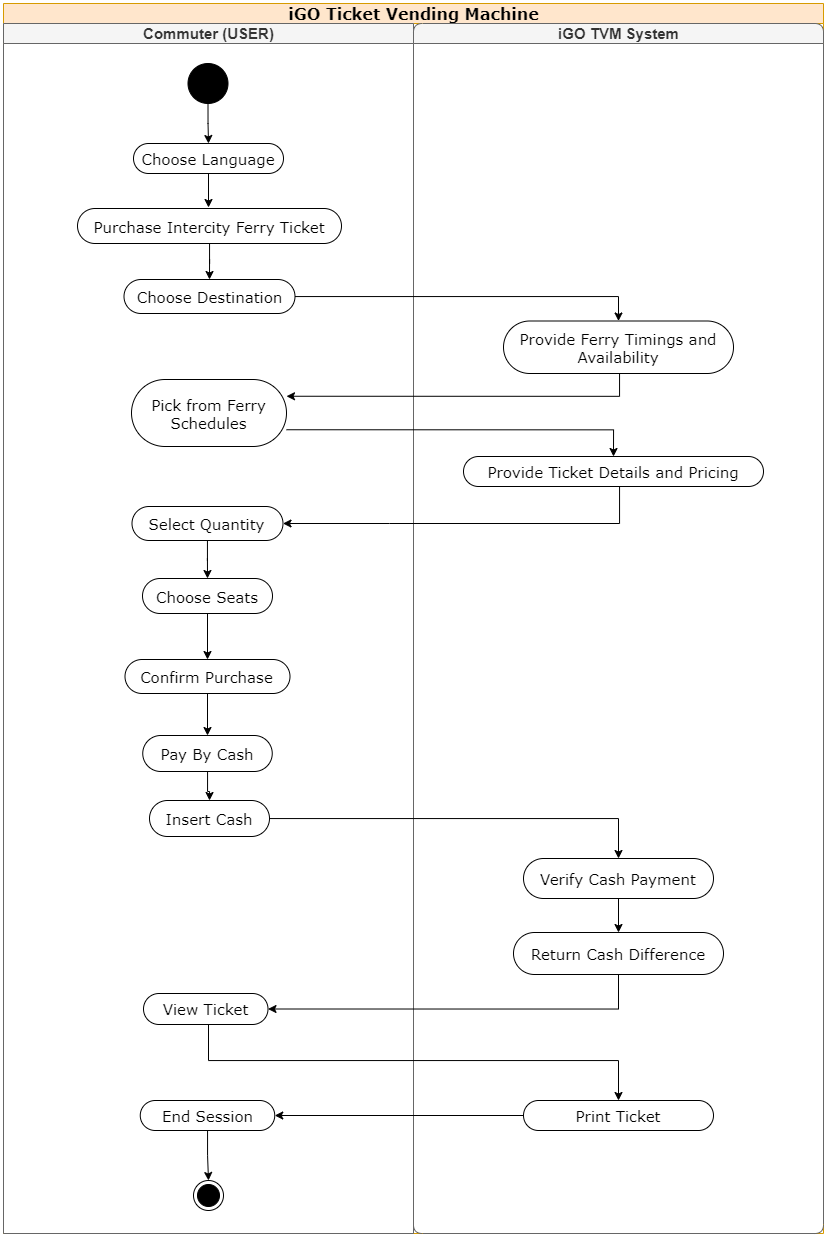
\includegraphics[width=\textwidth, height=0.95\textheight, keepaspectratio]{ActivityDiagrams/AD - 3.png}
    \caption{Activity Diagram for Cash Payment}
    \label{fig:ActivityDiagram_Cash}
\end{figure}
\clearpage

 \subsection{Pay by Card \emph{(Figure \ref{fig:ActivityDiagram_Card})}}
This activity diagram illustrates the process of purchasing a Montreal Ferry ticket using the iGo TVM System's {\bf Pay By Card} payment method. The process starts with the commuter selecting a language and choosing to purchase a ticket for the Montreal ferry. The system displays the available ticket types and their prices, and the commuter selects a ticket. After confirmation, the commuter inserts their debit/credit card and verifies their identity with a PIN. The bank then verifies the payment information and approves or declines the payment. Once the transaction is complete, the card is returned, and the commuter can choose to view the ticket, which the system can print or send via email to conclude the session.
\vspace{\baselineskip}

\begin{figure}[ht]
    \centering
    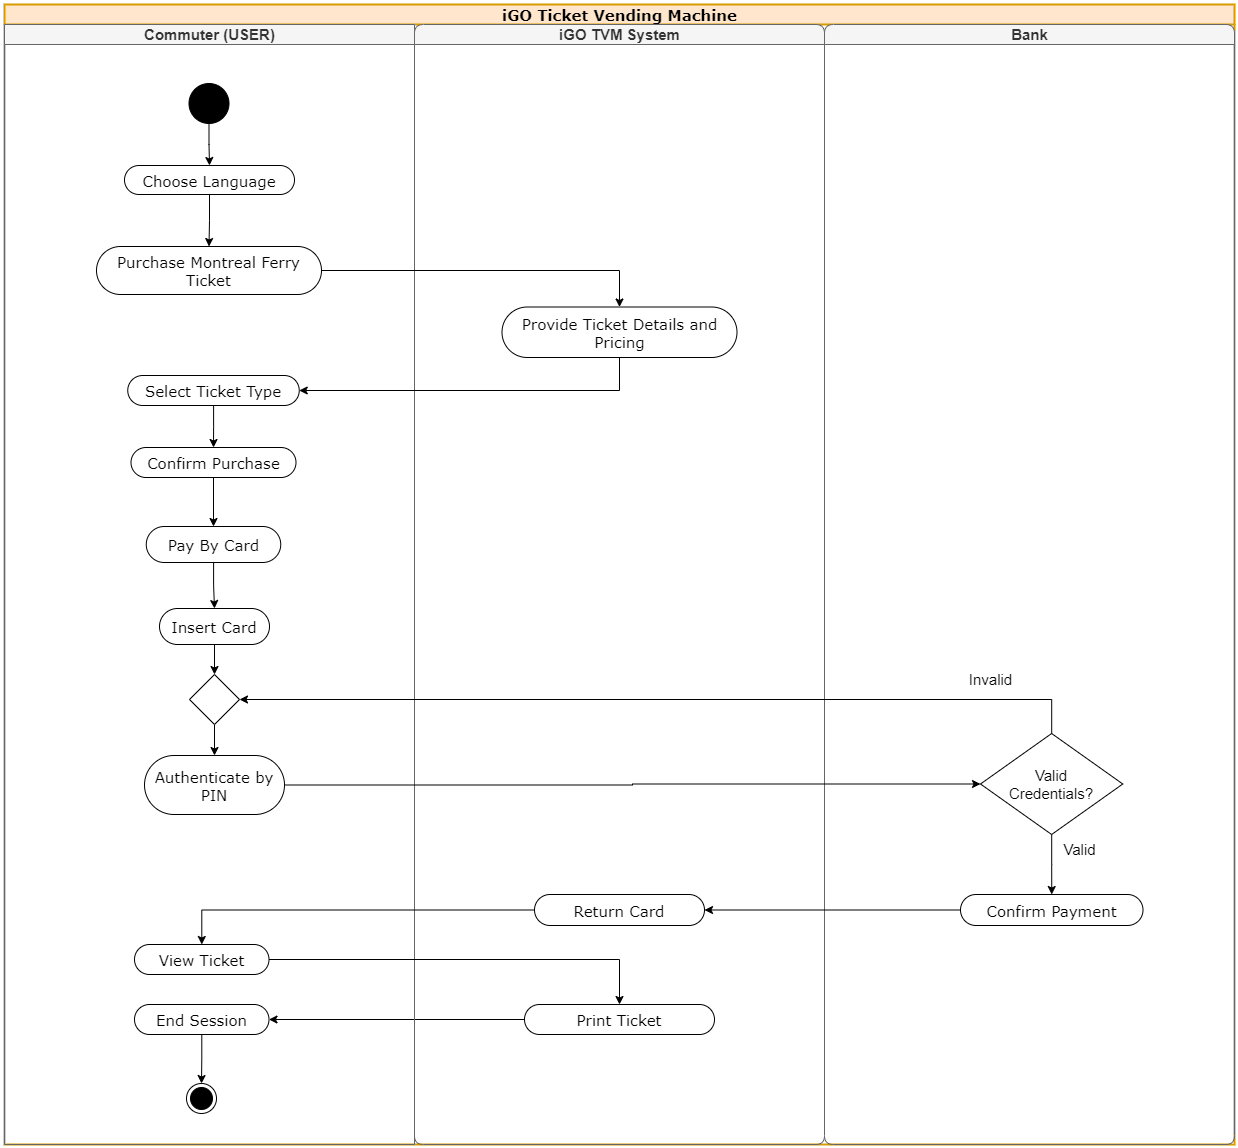
\includegraphics[width=\textwidth, height=0.7\textheight, keepaspectratio]{ActivityDiagrams/AD - 4.png}
    \caption{Activity Diagram for Card Payment}
    \label{fig:ActivityDiagram_Card}
\end{figure}
\clearpage

 \subsection{Cancel Booking Session \emph{(Figure \ref{fig:ActivityDiagram_Cancel})}}
The activity diagram depicts the activity flow for the cancellation of the ticket booking session before actual purchase. A commuter chooses the preferred language, and tries to purchase an Intercity ferry ticket by choosing destination, time, quantity, and seat. But then {\bf Ends Session} abruptly, before moving to the payment section. In activity flow occurs when the user decides not to purchase a ticket.
\vspace{\baselineskip}

\begin{figure}[ht]
    \centering
    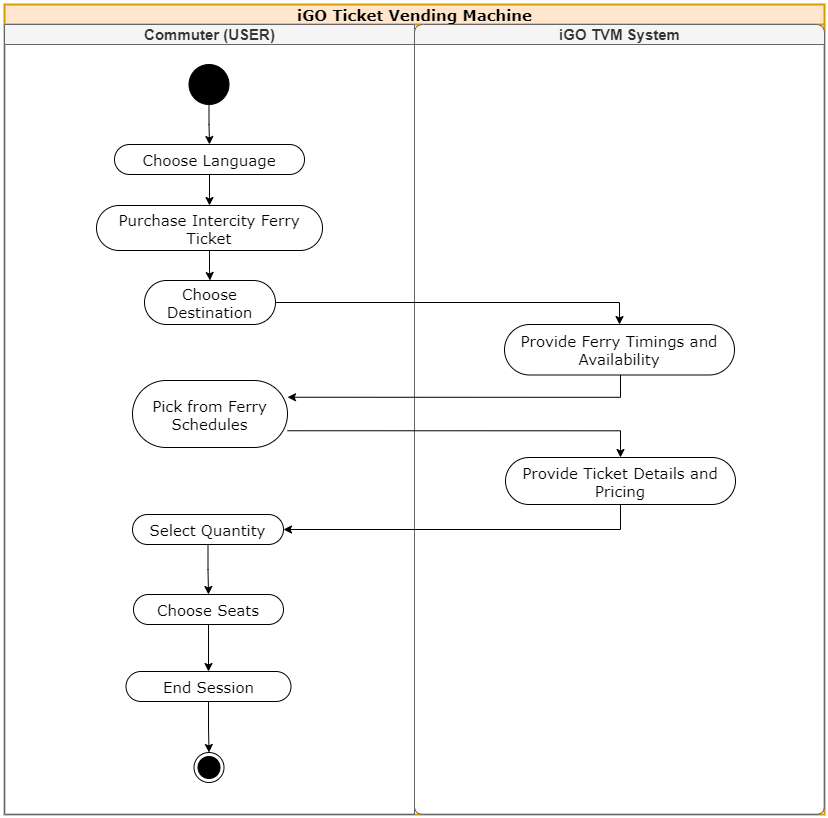
\includegraphics[width=\textwidth, height=0.73\textheight, keepaspectratio]{ActivityDiagrams/AD - 5.png}
    \caption{Activity Diagram for Cancellation before Payment}
    \label{fig:ActivityDiagram_Cancel}
\end{figure}
\clearpage

\subsection{Purchase Montréal Ferry Ticket \emph{(Figure \ref{fig:ActivityDiagram_Montreal})}}
The activity diagram depicts the activity flow of {\bf Montréal Ferry ticket} purchase process. The commuter chooses the preferred language, and then selects the ticket type from the ticket details \& prices displayed by the iGO TVM System. Then after confirmation, the commuter completes the payment by either cash or card mode. Upon successful payment, the commuter views and receives a ticket physically or digitally based on their choice. 
\vspace{\baselineskip}

\begin{figure}[ht]
    \centering
    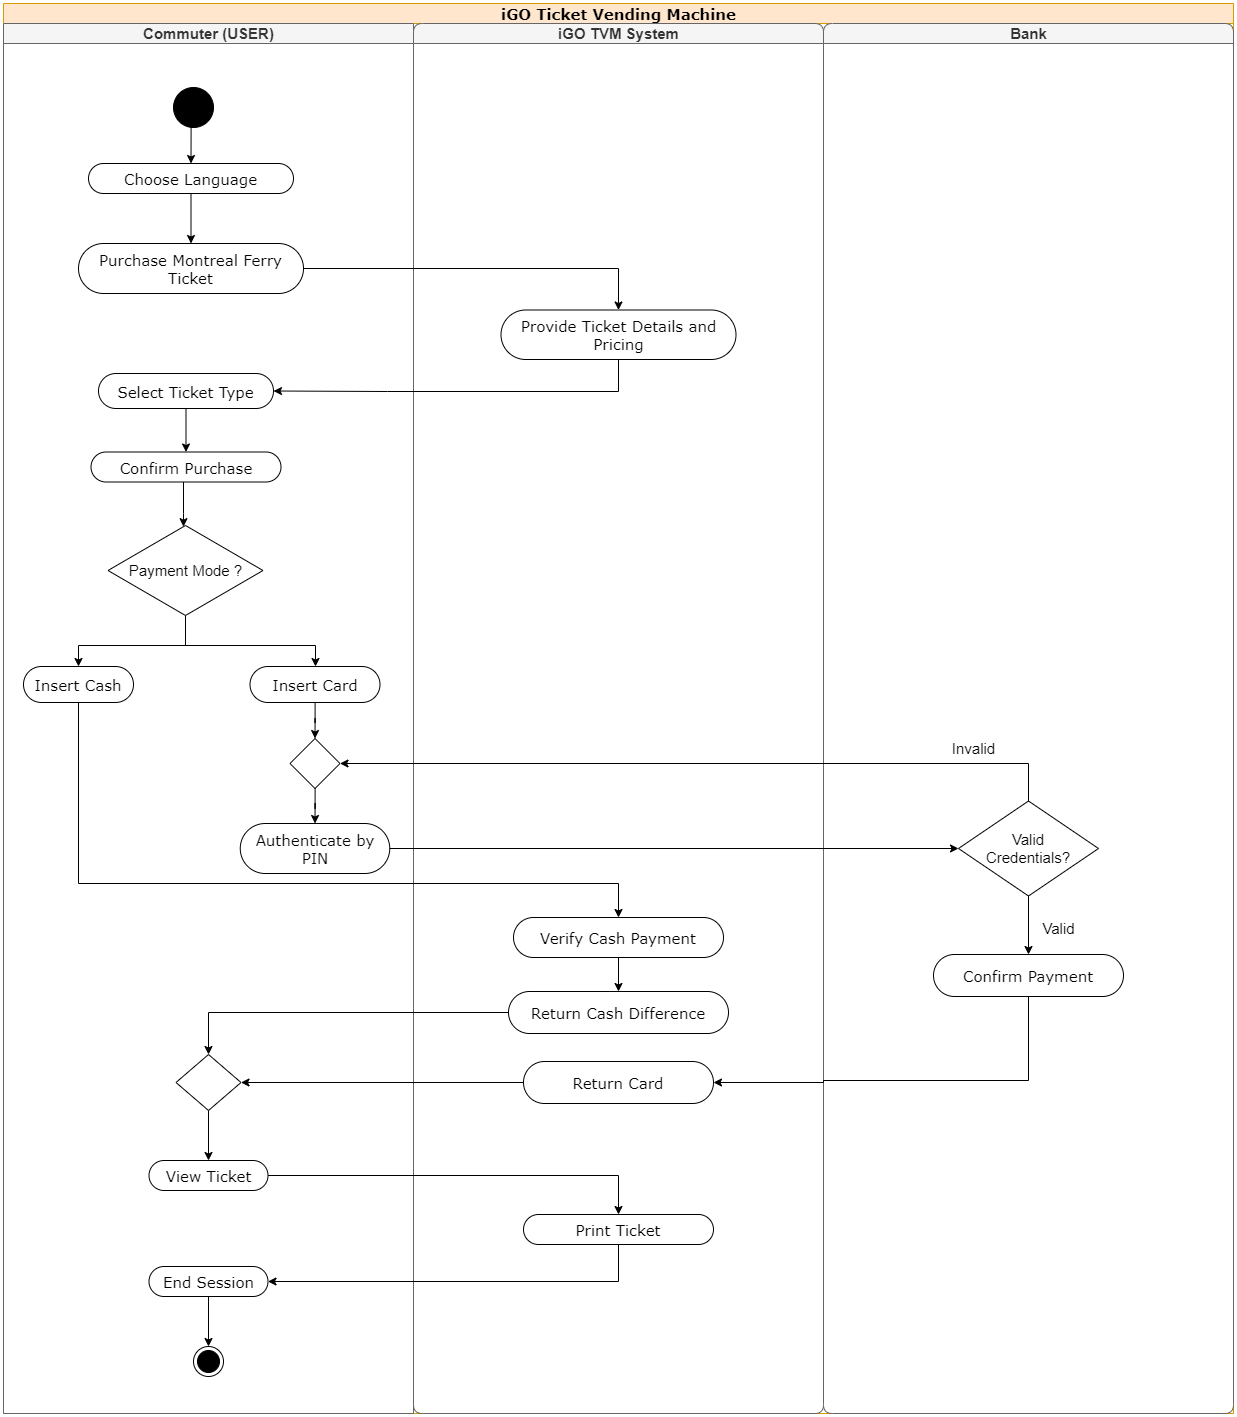
\includegraphics[width=\textwidth, height=0.73\textheight, keepaspectratio]{ActivityDiagrams/AD - 1.png}
    \caption{Activity Diagram for Montréal Ferry Ticketing}
    \label{fig:ActivityDiagram_Montreal}
\end{figure}
\clearpage

 \subsection{Purchase Intercity Ferry Ticket \emph{(Figure \ref{fig:ActivityDiagram_Intercity})}}
The activity diagram depicts the activity flow of {\bf Intercity Ferry ticket} purchase process. A commuter chooses a preferred language, and then selects the destination city for the travel, the ferry time from a schedule displayed by the iGO TVM System. The commuter also selects the ticket quantity and seats before confirmation. The commuter then completes the payment by either cash or card. Upon successful payment, a commuter views and receives a ticket physically or digitally.

\begin{figure}[ht]
    \centering
    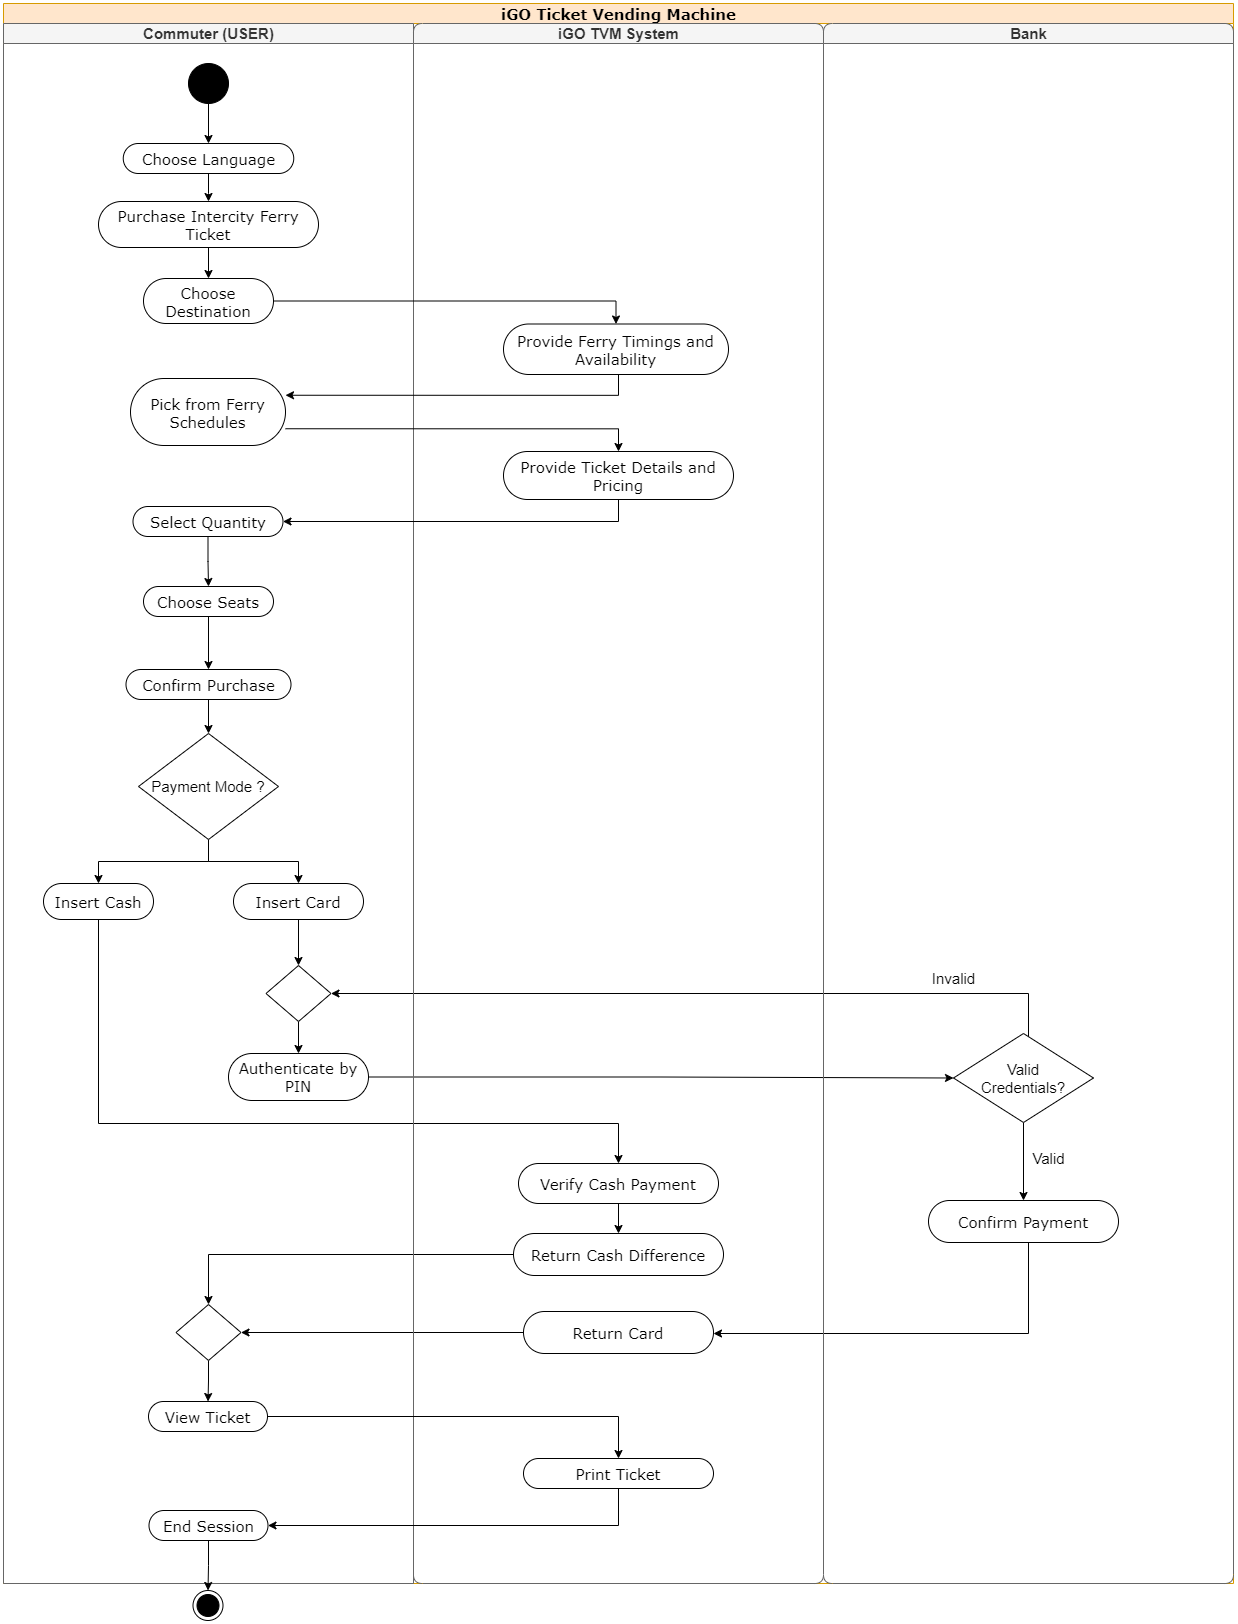
\includegraphics[width=\textwidth,
    height=0.735
    \textheight, keepaspectratio]{ActivityDiagrams/AD - 2.png}
    \caption{Activity Diagram for Intercity Ferry Ticketing}
    \label{fig:ActivityDiagram_Intercity}
\end{figure}
\clearpage


% \chapter{References}      %\begin{bibliography} creates its own page already.
\begin{thebibliography}{9}
\bibitem{TicketMachine}     %refer to this with \cite{TicketMachine}
Ticket machine. (2023, March 2). In Wikipedia.\\
\url{https://en.wikipedia.org/wiki/Ticket\_machine}.

\bibitem{ActivityDiagram}
Activity Diagram. (2023, March 5). In Wikipedia.\\
\url{https://en.wikipedia.org/wiki/Activity\_diagram}.

\bibitem{UIgoals}
Kersten M., (2021, January 25). \textit{4.Usability goals, UX design principles and factors} [PDF slides], Computer Science and Software Engineering, Concordia University.

\bibitem{DomainModelDiagramming}
Kamthan P., (2023, March 6). \textit{Introduction to Domain Modeling} [PDF], Computer Science and Software Engineering, Concordia University. \url{http://users.encs.concordia.ca/~kamthan/courses/soen-6461/domain_modeling_introduction.pdf}

\bibitem{UseCaseDiagramming}
Kamthan P., (2023, March 6). \textit{Introduction to Use Case Modeling} [PDF], Computer Science and Software Engineering, Concordia University. \url{http://users.encs.concordia.ca/~kamthan/courses/soen-6461/use_case_modeling_introduction.pdf}

\bibitem{MindMap}
Kamthan P. \textit{BRAINSTORMING AND MIND MAPPING} [PDF], Computer Science and Software Engineering, Concordia University. \url{https://users.encs.concordia.ca/~kamthan/courses/soen-6461/brainstorming_mind_mapping.pdf}

\bibitem{The Easy Guide to UML Activity Diagrams}
The Easy Guide to UML Activity Diagrams (2022, November 29)
\url{https://creately.com/guides/activity-diagram-tutorial/}

\bibitem{Use Case Diagram Relationships}
Use Case Diagram Relationships Explained (2022, December 13)
\url{https://creately.com/blog/diagrams/use-case-diagram-relationships/}

\bibitem{ROLE OF USE CASE DIAGRAM IN S/W DEVELOPMENT}
ROLE OF USE CASE DIAGRAM IN SOFTWARE DEVELOPMENT (2014, January)
% \url{https://www.researchgate.net/publication/322991847_role_of_use_case_diagram_in_software_development}
\href{https://www.researchgate.net/publication/322991847_role_of_use_case_diagram_in_software_development}{https://www.researchgate.net/publication/322991847\_role\_of\_use\_case\_diagram\_in\_software\\
\_development}      %circumvent warning

\bibitem{Formal Analysis Of Use Case Diagrams}
Formal Analysis Of Use Case Diagrams (2010, January)
\url{https://www.researchgate.net/publication/50365823_Formal_Analysis_Of_Use_Case_Diagrams}

\bibitem{Activity Diagram in UML: Symbol, Components & Example}
Activity Diagram in UML: Symbol, Components \& Example (2023, March 5). In guru99.\\
\url{https://www.guru99.com/uml-activity-diagram.html}.

\bibitem{Navettes Maritimes}
Navettes Maritimes (2023).\\
\url{https://navettesfluviales.com/en/}.

\end{thebibliography}

\appendix

\chapter{Interview Transcripts} \label{sec:Appendix_Interviews}
After the pilot interview, the three other interviews were conducted independently. Therefore, the format of the interviews may possibly not be consistent with each other. 
\subsubsection{Interviewee protection}
This goes without saying, but effort has been made to scrub out personal details in the interview (this includes the interviewee's real name). The transcripts here have been modified to protect the anonymity and confidentiality of the interviewed, and the interviewee is informed of this decision prior to the interview. No interviewee had been forcefully co-erced into giving an interview, and their consent has been acquired to record a transcript of the interview.

\section{Interview 1 (Pilot Interview)}
The transcript for the pilot interview was recorded live by keyboard strokes. Some information may be in shorthand or lost. The interview is conducted online.

\vspace{\baselineskip}
\noindent Interview 1\\
Interviewer : All members present. \\
Guest: Subject-1\\
\textbf{Transcript:}
\begin{enumerate}
    \item What features do you think are necessary in a ticket vending machine for public transportation?\\
Ans: For the vending machine itself, I’d like this machine to be easy to use, no queue for using it.
    \item So, How important is it for the vending machine to be user-friendly and easy to navigate on a scale of 1 to 10?\\
Ans: Umm, I'd say it's very important for the vending machine to be user friendly, as you won't be able to sell tickets faster.

Q: Okay That makes sense, But this is a very small , people will use this once a week or rarely for 5 mins , so do you think its as important?\\
Ans: We dont have a way to know that so its better 
    \item Do you think a touch screen interface or physical buttons would be more effective for a ticket vending machine an why?\\
	Ans: I personally like physical button, but I am aware touch interface becoming a fad recently\\
	Q: So, a touch interface will still be good for you right ?\\
Ans: I will be okay, but I would prefer physical buttons.
    \item Would you prefer a cash-only vending machine or one that accepts both cash and card payments?\\
Ans: Uhh, If it had to be one of the two, I would prefer card payments.

    \item What security measures do you think should be included in a ticket vending machine to prevent fraud or theft?\\
Ans: uhh, I think you are asking this to a wrong person.\\
	Q: Well what would you do ?\\
	Ans: Maybe have a security person standing next there. It might not be feasible but that's my answer. 
    \item How important is it for the vending machine to be accessible for people with disabilities, such as those who use a wheelchair or have visual impairments?\\
Ans: I mean ofc its important, it would be a good thing to get this machines accessible for people with disabilities.
    \item Would you prefer a standalone vending machine or one that is integrated with other transportation services, such as bus or train systems?\\
Ans: Umm, I mean, I am one to like it simple rather than integrated with other complex systems.
    \item Do you think it is important for the vending machine to have multilingual options for non-native speakers?\\
Ans: Yes, we are in Montreal, the two languages are English and French and considering other languages I don't have any particular preference but I wouldn’t favour that.
    \item How important is it for the vending machine to offer a variety of ticket options, such as single-use, day pass, or monthly pass?\\
Ans: Uh, I suppose it will be very convenient for people who like having the options. I would like to use single use tickets over the other choices.
    \item What do you think about the option to purchase tickets online and pick them up at the vending machine, rather than purchasing them directly from the machine?\\
Ans: Uhh personally, buying on site.
    \item How important is it for the vending machine to have real-time schedule and route information?\\
Ans: This is very convenient, I can know when I am late and can wait for the next ferry or vice versa in terms of hurry.
    \item Would you prefer a vending machine that prints physical tickets or one that allows for mobile ticketing options?\\
Ans: Uhh, I like the physical tickets rather than online.
    \item Do you think the vending machine should have a feature that allows for refunds or exchanges?\\
Ans: I would find that strange, I don't think this is a good idea.
    \item How important is it for the vending machine to be located in convenient areas, such as at major transportation hubs or in busy city centers?\\
Ans: I would think it has some advantages like compact, doesn’t take a lot of space. And the machines far from the ferry port will be inconvenient for me.
    \item Do you think it is important for the vending machine to have a customer service hotline for support?\\
Ans: I think it could be a good idea, but personally I have never used this kind of support .
    \item Would you prefer a vending machine that offers discounts or promotions for frequent users?\\
Ans: Umm, I mean you were already planning the monthly/day pass and that would be discount than normal price so it's fair.
    \item How important is it for the vending machine to be equipped with a camera for security purposes?\\
Ans: Uh, that’s a good question, security wise it’d be pretty good idea and for public location it's good.
    \item Do you think the vending machine should be able to accept contactless payments, such as Apple Pay or Google Wallet?\\
Ans: I personally, not in favour of contact less payment for security concerns.
    \item Would you prefer a vending machine that offers rewards or loyalty programs for frequent users?\\
Ans: Not personally, but I'm sure there are those in favor.
    \item How important is it for the vending machine to have a clear and visible display for ticket information and pricing?\\
Ans: Obviously very important.
    \item Do you think it is important for the vending machine to have a feature that allows for contactless ticket pickup, such as through a QR code or NFC technology?\\
Ans: Umm, I think physical ticket should be enough but if you could make it work than it could be good idea.
    \item Would you prefer a vending machine that offers a feature for pre-ordering tickets in advance of travel?\\
Ans: For me, advance ticket will be convenient.
    \item Do you think this specific Service(Ferry) needs a commuter card of some sort like Stm?\\
Ans: Right, if we dont use it often I suppose the ticketing system you have is fine.
    \item Do you think the vending machine should have a feature for scheduling or reserving seats on a ferry?\\
Ans: I dont reserving seats is a good idea, unless maybe it's like first class or economy class.
    \item How important is it for the vending machine to have a feature for live updates on service disruptions or delays?\\
Ans: Uhh, we have that similar ques before, i think that it would be good for providing updates which I can see on machine screen.
    \item How important is it for the vending machine to have a clear and easy-to-understand pricing structure for tickets?\\
Ans: uh,, I dont think its very important but the simplicity will make it easier to book tickets for me.
    \item Do you think it is important for the vending machine to have a feature for purchasing transit passes for a specific period of time, such as a month or a year?\\
Ans: yes, i dont use it often but people who uses very often will be good for them.
    \item How important is it for the vending machine to have a feature for purchasing?\\
Ans: For long distance, I’d say the comfort seats.
    \item Do you think it is important for the vending machine to have a feature for purchasing tickets for specific dates or times of travel?\\
Ans: Planning far ahead, but for people who wants to buy tickets in bulk that would be a good idea.
    \item Have you ever experienced any issues with the ferry/cruise service being overcrowded or not having enough space for passengers and/or cars?\\
Ans: Uhh before I used a ferry it was all good and enough space.
    \item How often do you use ferry/cruise services, and for what purposes?\\
Ans: I have used a ferry for a prom in high school.
    \item How much would you pay for a ticket for this ferry/cruise service?\\
Ans: Uh, I guess about \$5 would be fair price.
    \item What do you think about the option to purchase car tickets for the ferry/cruise service? Is it something you would use?\\
Ans: It is not the thing I would use but I am in favour our public transportation, but carrying a cars on ferry would be good idea.
    \item How often do you travel with a car when using the ferry/cruise service? Is it something you typically find convenient?\\
And: Ya, I don't use a car so not a good question for me.

\end{enumerate}

\newpage
\section{Interview 2}
The transcript was transcribed from an audio recording. The interviewee was assured that the audio recording would be deleted and not shared with anyone outside the interviewers, and that it is only to be used to write a transcript. At times, the audio is not clear due to poor mic quality, or loud noises. The interview is conducted online.

\vspace{\baselineskip}
\noindent Interview2:\\
Interviewer : Elvin, Kevin \\
Guest: Subject-2\\
\textbf{Transcript:}
\begin{enumerate}
    \item How important is it for a ticket vending machine to be able to accept multiple forms of payment, such as credit/debit cards, cash, and mobile payments?\\
Ans: For me,as far as I’m concerned, I like cashless payments, and, for that matter, contactless payment as well. So if there is Apple Pay, I would be very happy about it. 
    \item What features would you like to see in a ticket vending machine to make the ticket purchasing process more convenient?\\
Ans: Uhhh… A friendly user interface. English as the primary language. And, as I said, Cashless or contactless payment.
    \item What kind of security measures do you think should be implemented in a ticket vending machine to prevent fraud and theft?\\
Ans: Hmm.. I believe that someone has to come every day to ensure no one has installed a mask on the keypad, on the payment interface, that it records the payment details. It records strokes on a key.\\
Q: A key logger?\\
Ans: Yes, make sure there are no key loggers, especially in the payment interface-- the card payment.
    \item How important is it for a ticket vending machine to have a user-friendly interface for purchasing tickets?\\
Ans: I believe [it is] very important. The easier the better. Easier with fewer steps.
    \item Should a ticket vending machine offer the ability to print physical tickets, or should it only provide digital ticket options?\\
Ans: A bit of both, I prefer a digital ticket, but there are people who might want physical tickets for proof of travel, for business meetings.
    \item What types of tickets would you like to see offered in a ticket vending machine, such as single-use, day passes, or return trip tickets?\\
Ans: For a ferry, only single use, or day pass. Sorry, not day pass, I mean a return pass.
    \item Should a ticket vending machine offer the ability to purchase tickets for multiple people, such as a family or group of friends?\\
Ans: Yes, it’s more convenient as it will… it frees up lines.
    \item How important is it for a ticket vending machine to offer discounts or promotions for certain types of tickets or during certain times of the year?\\
Ans: Ya, it will be good to have discounts during vacation days, especially with some kind of recreational ticket.
    \item Should a ticket vending machine offer the option to purchase parking passes for those using the ferry/cruise service with a car?\\
Ans: In the ferry or outside the ferry station? You are asking for there to be a parking lot outside the ferry station. No, I think it complicates things.
    \item How important is it for a ticket vending machine to be available 24/7 for those who need to purchase tickets outside of normal business hours?\\
Ans: Aah, not important. I don’t think Ferry systems require pre-paid booking services.
    \item What kind of confirmation system should a ticket vending machine have to ensure that tickets are purchased successfully and accurately?\\
Ans: Uhh, once the quantity of tickets is… quantity of tickets are selected, just… Uhh… Confirm once the quantity and price, with tax.
    \item Should a ticket vending machine offer the ability to purchase tickets in advance, or only on the day of travel?\\
Ans: Only on the day of travel. For a ferry system, only on the day of travel.
    \item How important is it for a ticket vending machine to have a customer support system in case, uhhh… a u-- a user encounters issues while purchasing tickets?\\
Ans: Yes, it is important to have on-site assistance. On-site assistance would be better, rather than phone service, [because] you’ll have to call somebody.
    \item Should a ticket vending machine offer the ability to purchase tickets for multiple ferry/cruise routes or just one specific route?\\
Ans: Multiple routes.
    \item How important is it for a ticket vending machine to offer the ability to purchase tickets online or through a mobile app?\\
Ans: Actually, it’s a good feature to purchase online than through mobile.
    \item Should a ticket vending machine offer the ability to purchase tickets for multiple modes of transportation, such as buses or trains, in addition to ferries/cruise ships? The vending machines’ tickets, on top of boarding for ferries, should those also allow passage on other modes of transportations such as buses and trains?\\
Ans: Nah, no, nope. I would like the ferry system to be as simple as possible.
    \item Which type of payment confirmation options should a ticket vending machine offer, email or text message?\\
Ans: Text message.
    \item Should a ticket vending machine offer the ability to purchase tickets with a loyalty or rewards program?\\
Ans: Uhhh… Maybe, I don’t see how ferries… Maybe, maybe for a recreational ticket.
    \item How important is it for a ticket vending machine to have a clear and easy-to-understand pricing system for tickets?\\
Ans: I think it’s very important: the more simple it is the better.
    \item Should a ticket vending machine offer the ability to purchase tickets for both short- and long-distance ferry/cruise routes?\\
Ans: Yes.\\
Q: Would you like to expand on that?\\
Ans: Sure, okay sure. I think smaller routes need a different kind of interface, and the longer routes will need a different kind of [data?]..? Uhhh, but… The ability to purchase both [types of] tickets from the vending machine would be more convenient than to find the one vending machine that the uhh… to find the vending machine specific to your needs.
    \item How important is it for a ticket vending machine to offer the ability to purchase tickets for both one-way and round-trip travel?\\
Ans: I guess it’s important for me. It’s good. I-I-I, I will mostly take the ferry for roundtrip, so… I would like a round trip [ticket].
    \item Should a ticket vending machine offer the ability to purchase tickets in multiple languages for tourists and international travellers?\\
Ans: Yes, definitely. Especially in a famous city like Montreal, the ability to book in multiple languages would be good. Most, most importantly in English.
    \item How important is it for a ticket vending machine to offer the ability to purchase tickets for different seating classes or sections on the ferry/cruise ship?\\
Ans: For a long distance ferry, yes. For a short distance one, I think it would overcomplicate.
    \item Should a ticket vending machine offer the ability to purchase tickets with special accommodations for disabled or elderly passengers?\\
Ans: No. I believe the same tickets should be enough for both-- all kinds of passengers.
    \item How important is it for a ticket vending machine to have the ability to offer refunds or ticket cancellations in case of unexpected travel changes?\\
Ans: No, I don’t think refunds… Refunds are… I don’t think refunds are convenient in a vending machine. It should be done online or through customer service.
    \item Should a ticket vending machine offer the ability to purchase tickets for different age groups, such as children or seniors?\\
Ans: I think children under the age of 5 should get it for free, and uhh… Seniors over the age of… So are you asking me if it… about the tickets or the different price it should have..? Because it is a public transport, I believe that children under 5 and people over 65…\\
Q: What I mean is uhm… Uh, should they require to purchase… to make a purchase to board the ferry?\\
Ans: …No. The short distance ferry, no. But the long distance ferry should have a ticket, yes.
    \item How important is it for a ticket vending machine to have a clear and concise ticket selection process to prevent confusion for users?\\
Ans: It is extremely important. Very important. And uhh.. It determines if people will actually come back to the user interface and there will be problems-- if the user interface is not good, there will be more request in the customer care and uhh… The people who work behind the [inaudible, loud noise happened] will end up working more if the user interface is not good.
    \item Should a ticket vending machine offer the ability to purchase tickets for different time slots, such as morning or evening departures?\\
Ans: For the long distance, yes. For the short distance, no.
    \item Should a ticket vending machine offer the ability to purchase tickets with optional travel insurance?\\
Ans: Uhh, yes, it is good. Especially as it’s on water. It’s good to have insurance.\\
Q: How much would you pay for the extra insurance?\\
Ans: Short distance, maybe \$1. Long distance, \$5 to \$10… Not even \$10, maybe \$5 to \$7.
    \item How often do you use ferry/cruise services, and for what purposes?\\
Ans: I don’t use them often, but I have uhh, used ferries, ferries for [inaudible] and uhh.. It’s, it’s mostly for recreational purposes and not for like a [baby?] purpose. So I’m not sure I can… I’m not, I’m not the perfect person to talk about the [baby?] ferry, but the recreational one… Yeah.
    \item Uhh, how much would you pay for a ticket uhh, of[sic.] this ferry/cruise service? \\
Ans: Do you mean the short distance, or the long distance?\\
Q: Any ticket.\\
Ans: Short distance, maybe like \$4, \$5, \$4-\$5. Uhh, for the recreational one, mayyyyeah.. 20\$ or \$15. And for the long distance one from here to Toronto, probably, like, \$50, \$30, \$30 to \$50
    \item How do you usually purchase tickets for ferry/cruise services? Do you prefer buying tickets in advance or on the day of travel?\\
Ans: For the short distance one, on the day of travel. For the long distance one, maybe post-booking, but no request.\\
Q: Uhh, How do you usually purchase?\\
Ans: On the day of travel.
    \item What do you think about the option to purchase car tickets for the ferry/cruise service? Is it something you would use?\\
Ans: I don’t have a car now, but if I had a car, I would definitely.\\
Q: You would definitely?\\
Ans: Yes.
    \item How often do you travel with a car when using the ferry/cruise service? Is it something you typically find convenient?\\
Ans: I don’t have a car right now. I have only travelled on a ferry with a car like once, or twice maybe..? Not often.
    \item How do you typically plan your ferry/cruise trips? Do you find it easy to access the schedule and plan accordingly?\\
Ans: I have never faced a lot of difficulties, in that regard. But uhh, you should probably ask [inaudible, a different result?]…
    \item What do you think about the ticket vending machines located at, uhh, each stop? What would make them easy to use?\\
Ans: Yes, definitely. You should have a ticket vending machine at every stop. At every ferry pass.
    \item Have you ever used a recreational ticket for a ferry/cruise service before? Uhh, if so, what did you think about the experience?\\
Ans: Yes. It was very nice. Uhh.. When it’s recreational, it’s very fun. So I would prefer more emphasis on the recreational part of the experience than the daily commute.

Q: Thank you for your time.
\end{enumerate}

\newpage
\section{Interview 3}

Interview3:\\
Interviewer : Himanshu, Swapnil \\
Guest: Subject-3\\
\textbf{Transcript:}
\begin{enumerate}
\item \emph{Interviewer:} Hello, I hope you are doing good, just wanna ask some question about our iGo vending machien. What do you think about the recreational ticket option, where the ferry makes a circle and starts and ends at the same station? Is it something you would be interested in?\\
\emph{Interviewee:} As a customer, I think the recreational ticket option sounds like a great idea. It would provide a unique way to experience the beauty of Montreal and its surroundings while enjoying a relaxing ferry ride. I would definitely be interested in this option, as it would allow me to explore the city from a different perspective and make for a fun outing with friends and family.
\item \emph{Interviewer:} What do you think about the option to scan a QR code for ticket entry, rather than manually entering an ID number?\\
\emph{Interviewee:} I think the option to scan a QR code for ticket entry is a great idea. It's much more convenient and efficient than manually entering an ID number, which can be time-consuming and prone to errors. With QR code scanning, the process is quick and seamless, making the overall ticket purchasing and entry experience much more pleasant.
\item \emph{Interviewer:} Have you ever experienced long lines or wait times when purchasing tickets or boarding the ferry/cruise ship?\\
\emph{Interviewee:} Yes, I have experienced long lines and wait times when purchasing tickets or boarding the ferry ship. It can be frustrating, but I understand that sometimes it's just part of the process. However, I appreciate any efforts made to streamline the ticket purchasing and boarding processes to minimize wait times and make the experience more enjoyable for passengers.
\item \emph{Interviewer:} What do you think about the overall design and layout of the ticket vending machines at the terminals?\\
\emph{Interviewee:}  I think the design and layout of the ticket vending machines should be simple and intuitive, with clear instructions and easy-to-use buttons. The interface should be visually appealing and easy to read, with prominent displays indicating prices, routes, and schedules. Additionally, the machines should be easily accessible and have clear signage to help customers locate them.
\item \emph{Interviewer:} How important is it for you to have access to a ferry/cruise service that offers both short- and long-distance travel options?\\
\emph{Interviewee:}  Uhh, it's very important for me to have access to a cruise service that offers both short- and long-distance travel options. This allows for more flexibility and convenience in travel planning, and it's great to have the option to explore different destinations without having to switch between different modes of transportation.
\item \emph{Interviewer:} Have you ever experienced any issues with the TVM schedule not being accurate or up-to-date?\\
\emph{Interviewee:}  Yes, I have experienced issues with the TVM schedule not being accurate or up-to-date in the past. It can be frustrating to rely on the schedule and find out that the information is incorrect, leading to missed or delayed travel plans. It would be great if the iGo vending machine software could ensure that the schedule is always up-to-date and reliable to avoid these issues.
\item \emph{Interviewer:}How important is it for you to have access to a ferry/cruise service that offers a variety of ticket options, rather than just one type of ticket?\\
\emph{Interviewee:} Umm, it's important for me to have access to a ferry/cruise service that offers a variety of ticket options. This allows me to choose the ticket that best suits my travel needs and budget. Having multiple ticket options can also help to make the ticket purchasing process more flexible and convenient.
\item \emph{Interviewer:}What do 
you think about the option to purchase a return trip ticket for two directions, rather than having to purchase two separate tickets?\\
\emph{Interviewee:}  I think it would be great if the iGo vending machine software offered the option to purchase a return trip ticket for two directions. It would save me time and effort by not having to purchase two separate tickets. Plus, it would provide a convenient and hassle-free experience for passengers, which is always appreciated when traveling.
\item \emph{Interviewer:}How do you typically find out about any changes or updates to the ferry/cruise service schedule or system?\\
\emph{Interviewee:}   I would appreciate receiving updates about changes to the ferry/cruise service schedule or system through multiple channels such as email, SMS, or push notifications on the iGo ticket vending machine. Having access to up-to-date information in real-time would greatly help me plan my travel and avoid any potential delays or inconveniences.
\item \emph{Interviewer:}What do you think about the customer service provided by the ferry/cruise service, such as staff friendliness and helpfulness?\\
\emph{Interviewee:}As a customer, I value friendly and helpful customer service from ferry/cruise staff. It's important for staff to be approachable and willing to assist passengers with any questions or concerns they may have. A positive customer service experience can greatly enhance the overall travel experience, making passengers more likely to use the service again in the future.
\item \emph{Interviewer:} How important is it for you to have access to a ferry/cruise service that operates year-round, rather than only during certain seasons?\\
\emph{Interviewee:} Umm, it's crucial for me to have access to a ferry/cruise service that operates year-round. I rely on this service for both business and personal travel, and having it available throughout the year provides me with greater flexibility and convenience. Additionally, it allows me to take advantage of travel opportunities whenever they arise, without having to worry about whether or not the ferry/cruise service is operating at that time.
\item \emph{Interviewer:} Have you ever experienced any issues with the ferry/cruise service being overcrowded or not having enough space for passengers and/or cars?\\
\emph{Interviewee:} Yes, I have experienced issues with overcrowding on ferry services. It can be uncomfortable when there isn't enough space for passengers and their belongings. It would be great if the iGo vending machine software could help alleviate these issues by streamlining the ticket purchasing process and ensuring that passengers have a smooth and stress-free travel experience.
\item \emph{Interviewer:} What do you think about the option to purchase a ticket that can be used for multiple trips, rather than just a single-use ticket?\\
\emph{Interviewee:}I think having the option to purchase a ticket that can be used for multiple trips is a great idea! It would save me time and effort since I wouldn't have to purchase a new ticket every time I travel. It would also be convenient for frequent travelers who use the ferry system regularly. Overall, I think it would be a very useful feature to have in the iGo vending machine software.
\item \emph{Interviewer:} How important is it for you to have access to a ferry/cruise service that offers Wi-Fi or other amenities while onboard?\\
\emph{Interviewee:}Um, well, I guess having access to Wi-Fi or other amenities on board a ferry or cruise would be pretty nice, but it's not necessarily a deal-breaker for me. It really depends on the length of the journey and what other options are available for entertainment or work. So, I would say it's moderately important, but not absolutely essential.
\item \emph{Interviewer:} Have you ever used the ferry/cruise service for commuting purposes, such as to get to work or school?\\
\emph{Interviewee:} Um, Yes, I have used ferry/cruise service for commuting purposes in the past. It was a decent experience, but sometimes the ticket purchasing process could be slow and inefficient. I hope that the iGo ticket vending machine software will make the process faster and more user-friendly.
\item \emph{Interviewer:} What do you think about the option to purchase a group ticket for 5, 7, or 8 seats in a car? Is it something you would use?\\
\emph{Interviewee:} Hmm, that's an interesting idea. I think the option to purchase a group ticket for 5, 7, or 8 seats in a car could be really useful for families or groups of friends traveling together. It would be convenient to be able to purchase all the tickets at once and ensure that everyone is seated together. Personally, I would definitely consider using this option if I were traveling with a group.
\item \emph{Interviewer:} How important is it for you to have access to a ferry/cruise service that offers accessibility accommodations, such as wheelchair ramps or audio announcements?\\
\emph{Interviewee:} Hmm, it's really important for me to have access to accessibility accommodations on a ferry or cruise service. Things like wheelchair ramps or audio announcements can make a huge difference in my ability to enjoy the experience and get around safely. So, I would say it's very important for me to have these types of accommodations available.
\item \emph{Interviewer:} Have you ever used the Ferry/Cruise Service system to travel to neighboring cities for recreational or tourist purposes?\\
\emph{Interviewee:} Um, no, I haven't actually used the Ferry/Cruise Service system before for any recreational or tourist purposes. But, I'm still interested in hearing more about how the iGo ticket vending machine software will work and how it will make the process of purchasing tickets more convenient and efficient.
\item \emph{Interviewer:} What do you think about the overall convenience and ease of use of the Ferry/ Cruise Service system?\\
\emph{Interviewee:} Hmm, well, I think the overall convenience and ease of use of the Ferry/Cruise Service system could be improved. Sometimes it can be a bit confusing to figure out how to purchase tickets, and the lines can be long and slow-moving. It would be great if there were more self-serve options, like vending machines, to make it quicker and easier to get tickets. And it would be nice if there were more clear signage and instructions to help passengers navigate the system.
\item \emph{Interviewer:} How important is it for you to have access to a ferry/cruise service that offers environmentally-friendly options, such as hybrid or electric ferries?\\
\emph{Interviewee:} Well, I think it's pretty important to have access to environmentally-friendly ferry/cruise options, like hybrid or electric ferries. I mean, we all need to do our part to help protect the planet, right? Plus, it's just nice to know that you're doing something good for the environment while you're traveling. So yeah, I'd say it's definitely something I would consider when choosing a ferry/cruise service.
\item  \emph{Interviewer:} Alright, so that will be all from my side. Thank you for your suggestions and interactive conversation.
\end{enumerate}

\newpage
\section{Interview 4}

Interview 4:\\
Interviewer : Sadath, Himanshu \\
Guest: Subject-4\\
\textbf{Transcript:}
\begin{enumerate}
    \item \emph{Interviewer:} Hi, Interviewee. I'd like to start by asking how often you use ferry/cruise services and for what purposes?\\
\emph{Interviewee:} I have used ferry services a couple of times since I have been here in Montreal. I have used it for sightseeing and to hang out with friends just to explore around. 
    \item \emph{Interviewer:} How much do you usually pay for a ticket for this ferry/cruise service and do you think the amount is justified?\\
\emph{Interviewee:} I have usually paid around \$8 for the ticket and I think the price is pretty justified for the amount of pleasure and peace it brings to me at such a great price.
    \item \emph{Interviewer:} What features do you think are necessary in a ticket vending machine for public transportation?\\
\emph{Interviewee:} Some of the features which I could think of are route information, variety of ticket options, contactless payment option like Apple Pay and real time updates of the transport schedule.
    \item \emph{Interviewer:} Some may argue that a ticket vending machine is not very important since it is a small machine that people may use only once a week or rarely for a few minutes. What do you think about this?\\
\emph{Interviewee:} Vending machines are a good alternative to the traditional standing in queue for purchasing a ticket system. As there is no human interaction required people can purchase a ticket within their own comfort with multiple choice of payment modes. Although it doesn't really solve a bigger problem in the system, it is good to have them on the side.
    \item \emph{Interviewer:} On a scale of 1 to 10, how important is it for the vending machine to be user-friendly and easy to navigate? \\
\emph{Interviewee:} I think the sole purpose of vending machines is to ease the overall process of getting the tickets without hassling too much by standing in long queues so on that scale it should be definitely 10.
    \item \emph{Interviewer:} In your opinion, would a touch screen interface or physical buttons be more effective for a ticket vending machine, and why?\\
\emph{Interviewee:} A touch screen interface might be more fascinating to look at, but a physical button interface does have its own advantages and one of the most important advantages is that it can easily be operated by someone who is visually impaired or blind.
    \item \emph{Interviewer:} Would you prefer a vending machine that only accepts cash or one that accepts both cash and card payments?\\
\emph{Interviewee:} Well the more choices, better it is. A lot of times you don't carry cash or I personally use my phone wallet to pay at different places so definitely I would prefer both cash and card payments.
    \item \emph{Interviewer:} What security measures do you think should be included in a ticket vending machine to prevent fraud or theft?\\
\emph{Interviewee:} Some of the security measures which I could think of are security cameras or maybe an anti theft alarm which will be triggered based on force sensors input.
    \item \emph{Interviewer:} Do you prefer a standalone vending machine or one that is integrated with other transportation services, such as bus or train systems?\\
\emph{Interviewee:} I would prefer a dynamic vending machine which can be used for multiple services. Although I think it can be difficult or confusing to operate, but if designed perfectly it can really solve the hassle of going to different machines to get things done.
    \item \emph{Interviewer:} How important is it for the vending machine to offer a variety of ticket options, such as single-use, day pass, or monthly pass?\\
\emph{Interviewee:} It is really important as it covers wider range of people. There might be some people who are tourists or they just want to try the service once so they don't have to pay the full amount of the ticket, on the other side if there is someone who travels many times a month, can get a discounted monthly pass and save some money through that.
    \item \emph{Interviewer:} What do you think about the option to purchase tickets online and pick them up at the vending machine, rather than purchasing them directly from the machine?\\
\emph{Interviewee:} I don't think it will make much of a difference as anyways you will have to go and pick up the ticket from the vending machine.
    \item \emph{Interviewer:} How important is it for the vending machine to have real-time schedule and route information?\\
\emph{Interviewee:} It is really important because as a customer I would like to know about all this information before I go in myself to make sure if we are not running late or the kind of route we are going for this time.
    \item \emph{Interviewer:} Would you prefer a vending machine that prints physical tickets or one that allows for mobile ticketing options?\\
\emph{Interviewee:} I would prefer the mobile ticketing option as carrying a physical ticket along with you is an extra hassle and it can be easily misplaced or lost.
    \item \emph{Interviewer:} Do you think the vending machine should be able to accept contactless payments, such as Apple Pay or Google Wallet?\\
\emph{Interviewee:} I think definitely yes. As I personally use Apple pay to pay for most of my purchases, feature like that is really convenient. 
    \item \emph{Interviewer:} Do you think it is important for the vending machine to have a feature for purchasing tickets for specific dates or times of travel?\\
\emph{Interviewee:}  A feature for purchasing ticket for a specific date or time can be a really good additional feature which can be helpful but I dont think it’s that important as it may increase the complexity of the system and lead to more confusion.
    \item \emph{Interviewer:} How important is it for the vending machine to have a clear and easy to understand pricing structure for tickets?\\
\emph{Interviewee:} It is really important as the confusion related to price can end up with more unsatisfied customers which leads to bad user experience overall and as no person is going to be physically present at the location, customers can’t even get a quick solution for their price related issues which they may encounter because of confusion.
    \item \emph{Interviewer:} How important is it for the vending machine to have a feature for live updates on service disruptions or delays?\\
\emph{Interviewee:} It is very important as the person should be able to know before purchasing the ticket that if there is any delay or disruption in the service so that they can decide to proceed further accordingly.    
    \item \emph{Interviewer:} Do you think it is important for the vending machine to have a feature that allows for contactless ticket pickup, such as through a QR code or NFC technology?\\
\emph{Interviewee:} I think features like these could have come really in handy at the time of COVID 19 as we can make use of technology to enhance the machine with features such as these but I don't think it is really that important for a vending machine to have features like these.
    \item \emph{Interviewer:} Would you prefer a vending machine that offers rewards or loyalty programs for frequent users?
?\\
\emph{Interviewee:} Most definitely. This will encourage users to use these services even more and I personally would love to have offers like these where I am getting something in reward along with my time of using the services.
    \item \emph{Interviewer:} How important is it for the vending machine to be equipped with a camera for security purposes?\\
\emph{Interviewee:} A security camera can come in real handy when it comes to theft prevention and protection. There it is quite important that vending machine is equipped with camera.
    \item \emph{Interviewer:} Do you think this specific ferry service needs a commuter card of some sort like the STM’s OPUS Card?\\
\emph{Interviewee:} That would be a really good idea as for frequent travellers or people who use the services quite often, that could save some bucks and make it easy to use these services, overall enhancing the user experience. 
    \item \emph{Interviewer:} Do you think it is important for the vending machine to have multilingual options for non-native speakers?\\
\emph{Interviewee:} I think the vending machine should most likely have a multilingual options because there are a lot of immigrants and foreign international travellers who would love to enjoy the services but may get restricted because of language barrier.
    \item \emph{Interviewer:} How important is it for the vending machine to be accessible for people with disabilities, such as those who use a wheelchair or have visual impairments?\\
\emph{Interviewee:} I don't think it is going to make much of a difference for the vending machine to be accessible for people with disabilities especially for those who are on wheelchairs or have visual impairments. Instead, a person on duty might be able to help them even more than they can help themselves with the vending machine.

{Interviewers:} Thank you for your time.
\end{enumerate}

\end{document}
